\section{Designing Interactive Visuals for Dance from Body Maps: Machine Learning and Composite Animation Approaches}

The Latent Steps System described in the previous section is evaluated over a series of workshops and an artistic residency the resulted in a final performance. Participants were invited to experiment with the Latent Steps system, provide their feedback, and develop original works using it´s output. During the same course, we also trailed a non-generative visualisation method that instead calls upon a human animator to produce \textit{"Composite Animations"}. This would serve as an experimental benchmark to contrast with the usability and aesthetic affordances of the Latent Steps approach, as deemed by it's users. In this context, the performers and choreographer.

Throughout this comparison study, the terminolgy Machine Learning Interactive Visuals (MLIV) refers to the Latent Steps system while Compoisite Animation Interave Visuals (CAIV) represents an alternative non-generative approach.

\subsection{Introduction}

Authors such as Wechsler et al. \cite{wechsler_eyecon_2004}, Obermeier \cite{monteverdi_klaus_2007} and the OpenEndedGroup \cite{downie_choreographing_2005} have demonstrated the artistic potential of a creative exploration of interactive visuals in contemporary dance performances. Such interactive visuals consist of non-linear imagery, projected on stage, reacting to a specific input(s) in real time (e.g., the movement of dancers or cue-based triggering from an off-stage technician). There has been an increased attention to the role interactive visuals can play in relation to the audience. In a previous study, we identified design strategies for interactive visuals in dance performances aimed towards higher audience engagement \cite{correia_connected_2021}. As a way of fostering a deeper connection between the audience and dancers, authors such as Sugawa et al. \cite{sugawa_boiling_2021} have recently started to explore the use of biosignal data for interactive visuals. To reinforce this connection between audience and dancers, we follow a co-design process with dancers, to create with them the aesthetics and behaviour of the interactive visuals, to be shown to the audience.

According to our previous findings, in a study involving 10 professional dancers working with technology, a fruitful strategy to use technology in dance performances is to expose non-visible elements in the performance, namely the inner processes of the dancers – such as the thought process of dancers or their bodily data \cite{masu_how_2019}. For example, to convey the thought processes of dancers, technology could assist in revealing “what’s happening in the brain before the movement” or “the thinking process of someone doing something incredibly complex”. An example of revealing bodily data is the appropriation of biosensors (such as EEG, ECG and EMG sensors) by musicians to generate sound \cite{aly_appropriating_2021}. However, there is a lack of research on conveying the inner processes of the dancers during performances, through interactive visuals. In our research, we aim to make non-visible bodily elements apparent to an audience through interactive visuals, relying on the dancers’ somatic awareness during their practice.

\textcolor{red}{Lit Review}
Our approach is informed by the soma design process of Höök \cite{hook_designing_2018}, which “requires training your ability to aesthetically appreciate all your senses, but also to imagine through your senses, movements and material encounters” \cite{hook_soma_2019}. According to a soma design process, what takes form “is not only the digital and physical materials you use to build your interactive artifact with, but also the end-users’ somas”. 

We draw upon Höök's soma design process complimented with first-person principles granting a singularity bet designer and user \cite{hook_designing_2018}. We aim to involve the dancers (the ‘end users’ of the interactive visuals) in developing interactive visuals for performance that can expose non-visible elements. Dancers can be considered “somaesthetic connaisseurs”, following the terminology by Schiphorst \cite{schiphorst_self-evidence_2011}, which further highlights the importance of leveraging their soma expertise in co-designing the visuals, to achieve our aim of exposing non-visible elements. Tools used in soma design, such as body maps, are valuable in this study. Recent literature on soma design has aimed to overcome the temporal limitations of body maps, as “they exist as a snapshot or state representation” \cite{tennent_articulating_2021}. To solve this limitation, Tennent et al. propose the concept of “soma trajectories”: “how a user feels through an interaction, both in body and mind”  \cite{tennent_articulating_2021}.

Based on recent research on Machine Learning (ML) and autoencoders for generative visualization \cite{broad_autoencoding_2017, crnkovic-friis_generative_2016}, and in the use of ML for embodied interaction design \cite{plant_interactive_2021}, we identify potential in using ML to create interactive visuals for dance performance, from a corpus of body maps. Aly et al.’s research on appropriating biosensors for artistic purposes, identifying that “biosensing decodes inner structures of the performer’s body as a control variable” \cite{aly_appropriating_2021}, suggest that biosignal sensors can be useful to achieve our aim of revealing inner processes of dancers.

Our aim of exposing non-visible elements from the dancers leads to the following research question: \textit{how to design interactive visuals for contemporary dance performance, in a way that reveals the inner processes of the dancers?} Our hypothesis is: \textit{following a soma design process with dancers relying on body maps, combined with interactive technology and machine learning, can make non-visible bodily elements apparent, to be presented as interactive visuals.} To answer our research question, we devised a set of co-design stages involving two workshops with ten dancers each, and an artistic residency with two choreographers.

\subsection{Background}

\textcolor{red}{Lit Review}
\subsubsection{Dance, Biosignals and HCI}

The HCI community has been increasingly attentive to computational technology for dance, following a growing interest in embodied interaction. In this area, Fdili Alaoui et al. distinguished among categories of tools for: Generation (of new choreographic material); Interaction (in real time with performers on stage); Reflection (on choreography); and Annotation (tools assisting the creative process) \cite{fdili_alaoui_chiseling_2013}. Similarly, Raheb et al. categorized dance technologies into: Choreographic tools; Augmented performance; Education; Research and analysis; and Games  \cite{raheb_dance_2019}.  HCI research and technologies targeting choreographers and dancers have emerged across these areas, such as: development of tools and techniques for annotation \cite{cabral_multimodal_2011}; tools for documenting choreographic processes \cite{ciolfi_felice_knotation:_2018, ciolfi_felice_studying_2021}; real time interaction \cite{fdili_alaoui_chiseling_2013}; and choreography generation itself \cite{calvert_evolution_1993}., or augmented performance according to \cite{raheb_dance_2019}. Zhou et al. have recently conducted a systematic review of the past twenty years of dance literature in HCI \cite{zhou_dance_2021}. They identified four main categories of technological approaches: Physiological Sensing; Multisensory Perception; Movement Quality; and Agent Collaboration. Fdili Alaoui et at. created a methodology to combine multimodal capture with recognition of Laban Effort qualities \cite{fdili_alaoui_seeing_2017}. They distinguished among different approaches to collect information from the body: Positional data retrieved by motion capture; Movement dynamics recorded by inertial sensors; and Physiological information obtained from biosignal sensors. Rostami et al. \cite{rostami_bio-sensed_2017} created five design concepts for interactive performance adopting bio-sensing and bodily tracking technologies. Aly et al. conducted a review of biosensor modalities for performance with an HCI perspective, which discusses the affordances of muscular activity to depict rich movement information \cite{aly_appropriating_2021}. The different contexts of the studies by Rostami et al. and Aly et al. include not only dance but other performance areas as well (the latter focuses on music). The above authors highlight the use of biosignal sensors, one of the key technologies we use in our study, to collect data from the body.

\subsection{Interactive Visuals in Dance}

In the intersection between dance and HCI, interactive visuals have been the focus of recent research. Hsueh and colleagues investigated creativity in dance \cite{hsueh_understanding_2019}. They developed a series of interactive visuals, then invited dance practitioners to use those visuals to generate movement materials. Based on the results of this study, the authors developed a taxonomy composed of three different relationships and two movement responses between dancers and visuals. The classification is composed of six different “interaction patterns” organized in two domains: Relationship to Visuals; and Movement Type. In the Relationship to Visuals domain, there are three levels (Instrument, Partner and Medium). Instrument relates to manipulation of visual properties by the body, helping dancers form a first-person relationship. In Partner, the dancer establishes a dialogue with the visuals, which have an autonomous behavior. Finally, in the Medium level, visuals are used to communicate with other dancer(s), or between choreographer and dancer. We will use this taxonomy to discuss our findings.

We previously conducted an audience study on the experience of live visuals in dance, involving four different dance performances, each exploring a different approach for interaction involving visuals (motion capture, sensors, video camera and minimal interaction) \cite{correia_connected_2021}]. This allowed the authors to propose a mapping clarity diagram, as perceived by the audience, and a performance network diagram (with: the different actors; on stage components; and conceptual elements), for dance performances with interactive visuals. Sugawa et al. were able to sense cardiovascular and electrodermal activity from audience members and appropriate this sensor data to influence staging elements, such as visual projections, music, and lighting \cite{sugawa_boiling_2021} This allows the on-stage performers to react to the internal states of the audience according to the sensory data. This demonstrates how the visual representations of the body can be used to facilitate å non-verbal exchange between performer and audience. Although this this case, it focuses on the acquiring signals from the audience, whereas in our study, we focus on the dancers.

\subsubsection{Body Maps}

The term “body mapping” is defined as the process of creating body maps (human body images) “using drawing, painting, or other art-based techniques to visually represent aspects of people's lives, their bodies and the world they live in” \cite{gastaldo_body-map_2012}. Body mapping encourages embodied awareness and is also used as a knowledge production and translation strategy \cite{jager_embodied_2016}. Núñez-Pacheco and Loke introduced the concept of felt-sensing -- inner exploration of bodily feeling -- using body maps \cite{nunez-pacheco_felt-sensing_2016}. Núñez-Pacheco proposed “the use of tangible materials as a way to articulate experience from the inner self”, also employing body maps \cite{nunez-pacheco_tangible_2021}. In a scenario closer to the artistic research herein presented, Loke and Khut \cite{loke_intimate_2014} developed an art exhibition using “interactive heart rate controlled audio-visuals with audience participation”. They used body maps as a means for audience members to describe “sensations and images they experienced within and around their body, during the interaction” \cite{loke_intimate_2014}.

The body maps Gastaldo et al. presented in their research are free-form and unconstrained, there is no predefined structure (such as a preexisting body outline) and include contextual elements such as annotations. A more constrained body map, with an outline of the human body, is used by Windlin et al. \cite{windlin_soma_2019}, to reflect on experiences through drawings and notes: “these maps became a rich source of data for first-person perspectives of bodily experiences and sensations”. For the body maps, the authors adapted an earlier body outline from Loke et al. \cite{loke_bodily_2012}. A similar body map has been used in related soma design research, for example by Höök et al. \cite{hook_soma_2019} and Tsaknaki et al. \cite{tsaknaki_teaching_2019}. Nummenmaa et al. conducted a study on bodily sensations associated with different emotions, using body maps \cite{nummenmaa_bodily_2014}. Participants were shown two outlines of bodies alongside emotional words, stories, movies, or facial expressions, and they were asked to color the body regions whose activity they felt to be increased or decreased during the viewing of each stimulus. Based this review on body maps, we identify the use of more \textbf{free-form body maps} (such as the ones used in \cite{gastaldo_body-map_2012}) and \textbf{outline-based body maps} (such as the ones used in \cite{windlin_soma_2019} and \cite{nummenmaa_bodily_2014}). We adopt both types in our study.

\subsubsection{Machine Learning and Dance}

In terms of dance, Silang Maranan et al. developed an ML system that generates real time classifications of movement qualities using Laban Movement Analysis \cite{silang_maranan_designing_2014}. The system also generates abstract visualizations based on those classifications. Brenton et al. proposed interactive visualizations that react to the free-form movements, allowing to respond to “the idiosyncratic movements of an individual dancer”, using ML mapped to visuals \cite{brenton_embodied_2014}. Murray-Browne and Tigas proposed an open-ended mapping process (entitled “latent mapping”), leveraging an ML algorithm trained on a corpus of unlabelled gestural data \cite{murray-browne_latent_2021}. Plant et al. proposed a new tool based on interactive ML (\textit{InteractML}) to “make embodied interaction design faster, adaptable and accessible to developers of varying experience and background” \cite{plant_movement_2020}. In \textit{InteractML} “the user provides training examples (movement data), classifies these examples and can iteratively edit” those examples \cite{plant_interactive_2021}. These examples are relevant for us, as we aim to employ real time machine learning for dance.

A particular use case of ML in dance is the creation of an ‘artificial dancer’, projected on stage. McDonald and collaborators developed Discrete Figures, based on 40 separate motion capture recording sessions \cite{mcdonald_dance_2018}. Each session was composed of a dancer improvising in a different style (“robot”, “sad”, “cute”, etc) \cite{mcdonald_dance_2018}. This allowed to create a dataset of motion capture data, and from that a virtual “AI dancer”, with whom a real dancer establishes a dance dialogue with. Berman and James followed a similar logic, but based on real-time data \cite{berman_learning_2018}. They presented a system built for a dance performance, where an autoencoder neural network is trained in real time with motion data captured live on stage. This allows to generate an “artificial performer” projected on a screen and “enabling a mutual exchange of movement ideas” between “artificial” and “human” dancers \cite{berman_learning_2018}. The method employed in \cite{mcdonald_dance_2018} of different data capture sessions from dancers based on different sessions / themes of dance relates to how we conducted our own data capture, with five discrete sections / themes.

\subsection{Methods}

In this section, we present an overview of the study design and methods used. In the Design Stages and Evaluation Stages sections, these are further detailed.

\subsubsection{Study Design}

To answer our research question, we adopted a co-design perspective with dancers. To facilitate the co-design process, we relied on the different layers of appropriation exposed in the design-inuse model by Botero et al. \cite{botero_expanding_2010}: \textit{reinterpreting} possible uses of an artifact, \textit{adapting} and even \textit{reinventing} the artifacts, when some changes are operated on the artifacts (in collaboration with designers). We distributed the co-design process across four stages over six months (figure 1), in the scope of the project Moving Digits (https://movingdigits.eu): two participatory workshops with dancers; a technological development stage in between the workshops; and a final artistic residency. Throughout the process, we adopted different strategies to engage our participants in the design process.

Our \textbf{Stage 1} consisted of a sketching workshop (2 days), where ten dancers (see Participants section below) created movement exercises and then sketched body maps, based on those exercises. In \textbf{Stage 2}, our research team developed prototypes to create interactive visuals from the body maps generated, across three months. In \textbf{Stage 3} (4 days), the ten dancers tested our systems, and then provided feedback and suggestions, in two final focus group sessions (one per prototype). We used this feedback to iterate the respective designs. In the longer \textbf{Stage 4}, the systems were used to create, rehearse and present choreographies by two of the participants in the previous stages, leading to further evaluation (12 days in total, 6 days per participant). Although the design activities took place throughout the four stages, we will refer to Stages 1 and 2 as \textit{design stages}, as the main design features were created then; and Stages 3 and 4 as \textit{evaluation stages}, as we conducted iterative fine-tuning of our previous designs, while focusing on evaluation.

\begin{figure}[ht]
  \centering
  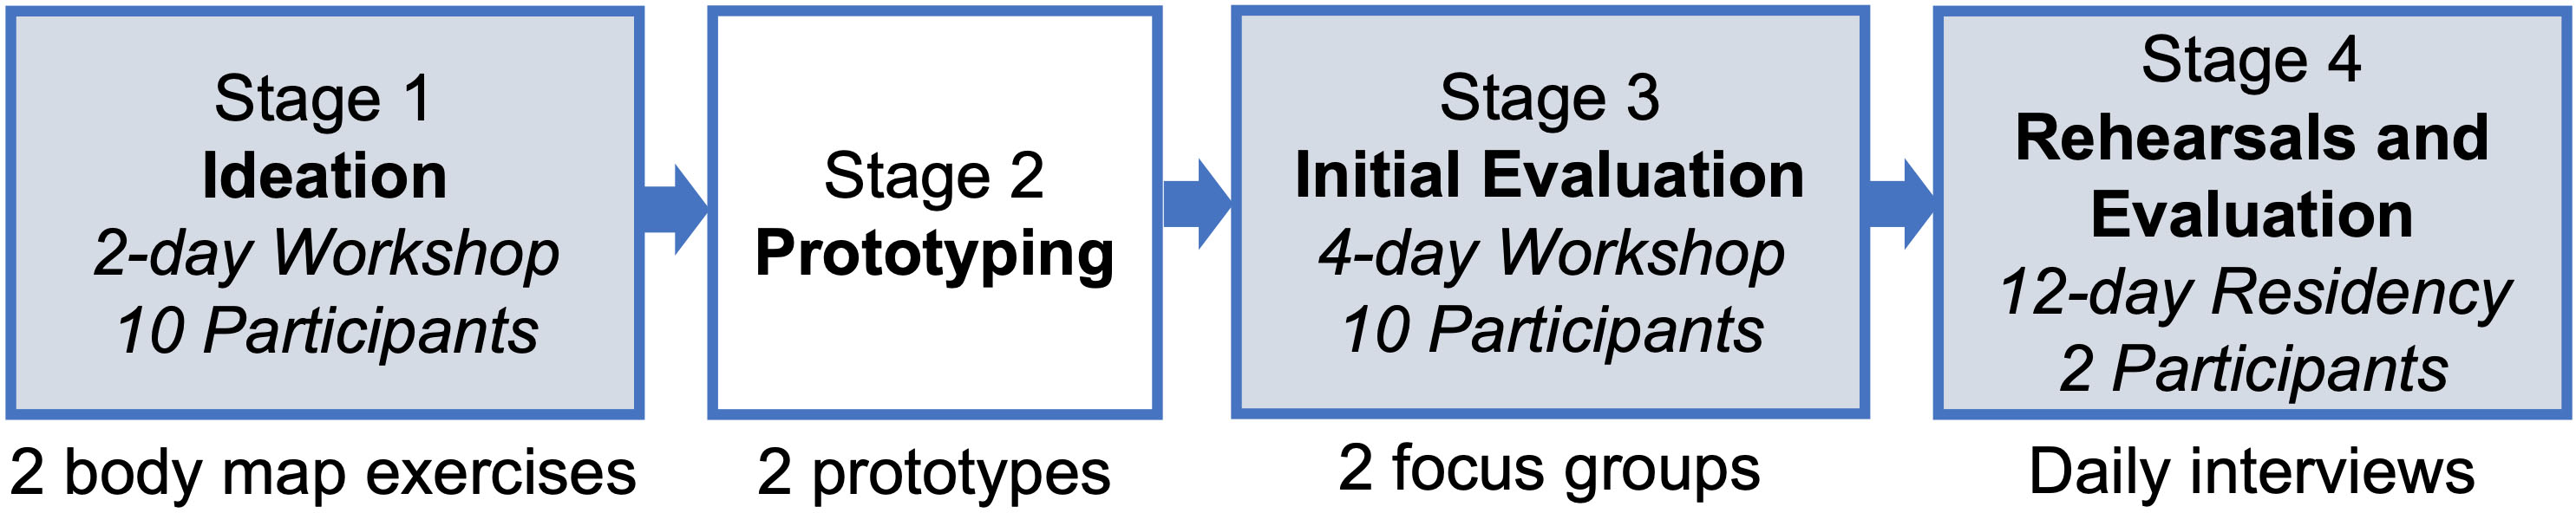
\includegraphics[width=0.9\linewidth]{Chapters/Figures/modi_dis/multistage.jpg}
  \caption{Diagram with stages of the research, over a six-month period}
    \label{fig:multistage}
\end{figure}
% Figure 1: Diagram with the four stages of the research, over a six-month period

\subsubsection{Data Collection and Analysis}

Movement exercises conducted in Stage 1 were video recorded and the respective biosignal data was collected (see Stage 1 section). We collected sketches from the dancers related to those exercises, using the two types of body maps identified in the Related Work section: \textit{free-form} and \textit{outline-based}. We asked dancers to annotate the body maps, following the approach by Gastaldo et al. \cite{gastaldo_body-map_2012}. These materials were scanned for use in the systems to be developed. Each dancer was asked to explain the body maps in their own worlds, to shed more light into the sketches – a body map \textit{testimonio}, using the terminology from Gastaldo et al.. The \textit{testimonios} were also video recorded.

In Stage 3, after the prototype development, we conducted two focus groups for the evaluation of both systems. In Stage 4, we conducted daily interviews with participants (across six days for each participant), for further evaluation and design iteration. These were audio recorded. The systematic data collection in Stage 4 is based on the technomethodology approach proposed by Dourish, involving the analysis of actions “moment-by-moment”, promoting a detailed analysis of actual practice \cite{dourish_where_2004} – adequate for the setting of choreography rehearsals. Therefore, we combined a shorter data collection and evaluation with more dancers (Stage 3), with a more extended and continuous evaluation, with fewer dancers (Stage 4).

The audio recordings of the two studies, in Stages 3 and 4 (focus groups and daily interviews, respectively), were transcribed and subjected to thematic analysis \cite{braun_using_2006}, independently. For each of the two thematic analyses, we coded the data using an inductive approach, and the codes were then organized into themes. We followed an inductive ‘bottom up’ approach to identify patterns within the data: “a process of coding the data without trying to fit it into a preexisting coding frame, or the researcher’s analytic preconceptions”. Therefore, in this process we were not driven by theory or the questions we asked. The analyses were conducted by the first author and cross-checked by the second. 

% We are aware that our profile as HCI researchers (particularly in the field of HCI) and also as artists ourselves may have influenced our interpretation of the data.  We used the software Atlas.ti (https://atlasti.com) to assist in the coding and analysis.

\subsubsection{Study Participants}

The two workshops involved a total of 12 international professional dancers in the field of contemporary dance, between 27 and 49 years old (11 female, 1 male), selected from an open call distributed to contemporary dance mailing lists (resulting in 92 applicants, 73 female, 19 male). 

Ten participants took part in the workshops on Stages 1 and 3. Two of the participants from Stage 1 could not attend the Stage 3 workshop due to scheduling issues, and were replaced by two other applicants from the initial open call. The two participants in Stage 4 (both female, 32 and 45 years old) were selected from the previous group of participants. The selection was based on a call for proposals, between Stages 3 and 4, targeting previous participants, to develop choreographies using the prototypes.

One reviewer of the corresponding publication critizised the gender imablance of the user group in respect to generizability. We may direct this to a higher number of female dance artists in the field of contemporary dance, and that the CVs of the male applicants were considered less fitted to the project than of the female applicants. It could even be commented that this effort actually poses to counter a historical overshadowing of non-male perspectives in Science and Technology Studies (STS) \cite{wajcman_feminist_2010,hook_soma_2019}.

\subsection{Design Stages}

\textcolor{red}{Move back to preliminary actions}
\subsubsection{Stage 1 - Sketching Workshop}

The first stage consisted of a two-day sketching workshop, which
took place at STL, a dance center in Tallinn, Estonia. The objective of this stage was to gather visual ideas and data about the dancers’ inner bodily processes during movement, to assist in the design and development of the interactive visuals systems for performance. Following approaches from our literature review, we used the two types of body maps identified (free-form and outline-based) as the main tool to collect visual ideas, and we used biosignal sensors to gather bodily data.

We decided to use biosignal sensors as one of the strategies toward our aim of revealing internal information from the dancer’s body. We used the BITalino R-IoT to acquire muscle activity, acceleration, and orientation data. The use of these sensing modalities is informed by the corresponding literature review, particularly in regards to stability and usablity during intense phyisical activity \cite{aly_appropriating_2021}.

The workshop involved three activities (the first on day 1, the other two on day 2):
\begin{enumerate}
    \item  The dancers prepared a movement exercise, consisting of five thematic sections, agreed upon collectively between them: Comfortable; Difficult; Undefinable; Aesthetic Form; and Open. Each dancer then created their own interpretation of the movement exercise, based on improvisation. This approach of combining improvisation with different, discrete, sections around a theme is similar (although smaller in scale) to the procedure followed by McDonald to generate an ML dataset for a dance piece \cite{mcdonald_dance_2018}.
    \item Each dancer was asked to perform the movement exercise, which was documented. The documentation consisted of video recordings and collection of biosignal data of each dancer. The data was labeled according to the dancer and to the section of movement exercise.
    \item The dancers drew body maps based on the movement exercise and their somatic impressions of it. We asked performers to create two types of drawings for each section of the choreography: free-form body maps and outline-based body maps (the two types of body maps identified in our Related Work section). We decided to have a range of more free-form and more constrained body maps in order to cover the different approaches identified in literature, and experiment with diverse designs for interactive visuals. Participants were given paper, colored felt pens and also clipboards for their drawings, so that they could move freely in the studio, and reenact the movements at will for accurate representation, while having the drawing materials at hand.
\end{enumerate}

The free-form body maps (figure \ref{fig:free-form-map}) resulted in very diverse and individual approaches. Each dancer produced five free-form body maps -- one per section. Following the approach by Gastaldo et al. \cite{gastaldo_body-map_2012}, we asked participants to annotate these body maps. In our case, the annotations were done in an overlay sheet, which was stapled to the main page for the drawing. That way, the drawings could be scanned independently of the annotations, in the future (e.g., for animation purposes). We also recorded video \textit{testimonios} of dancers explaining their body maps.

\begin{figure}[ht]
  \centering
  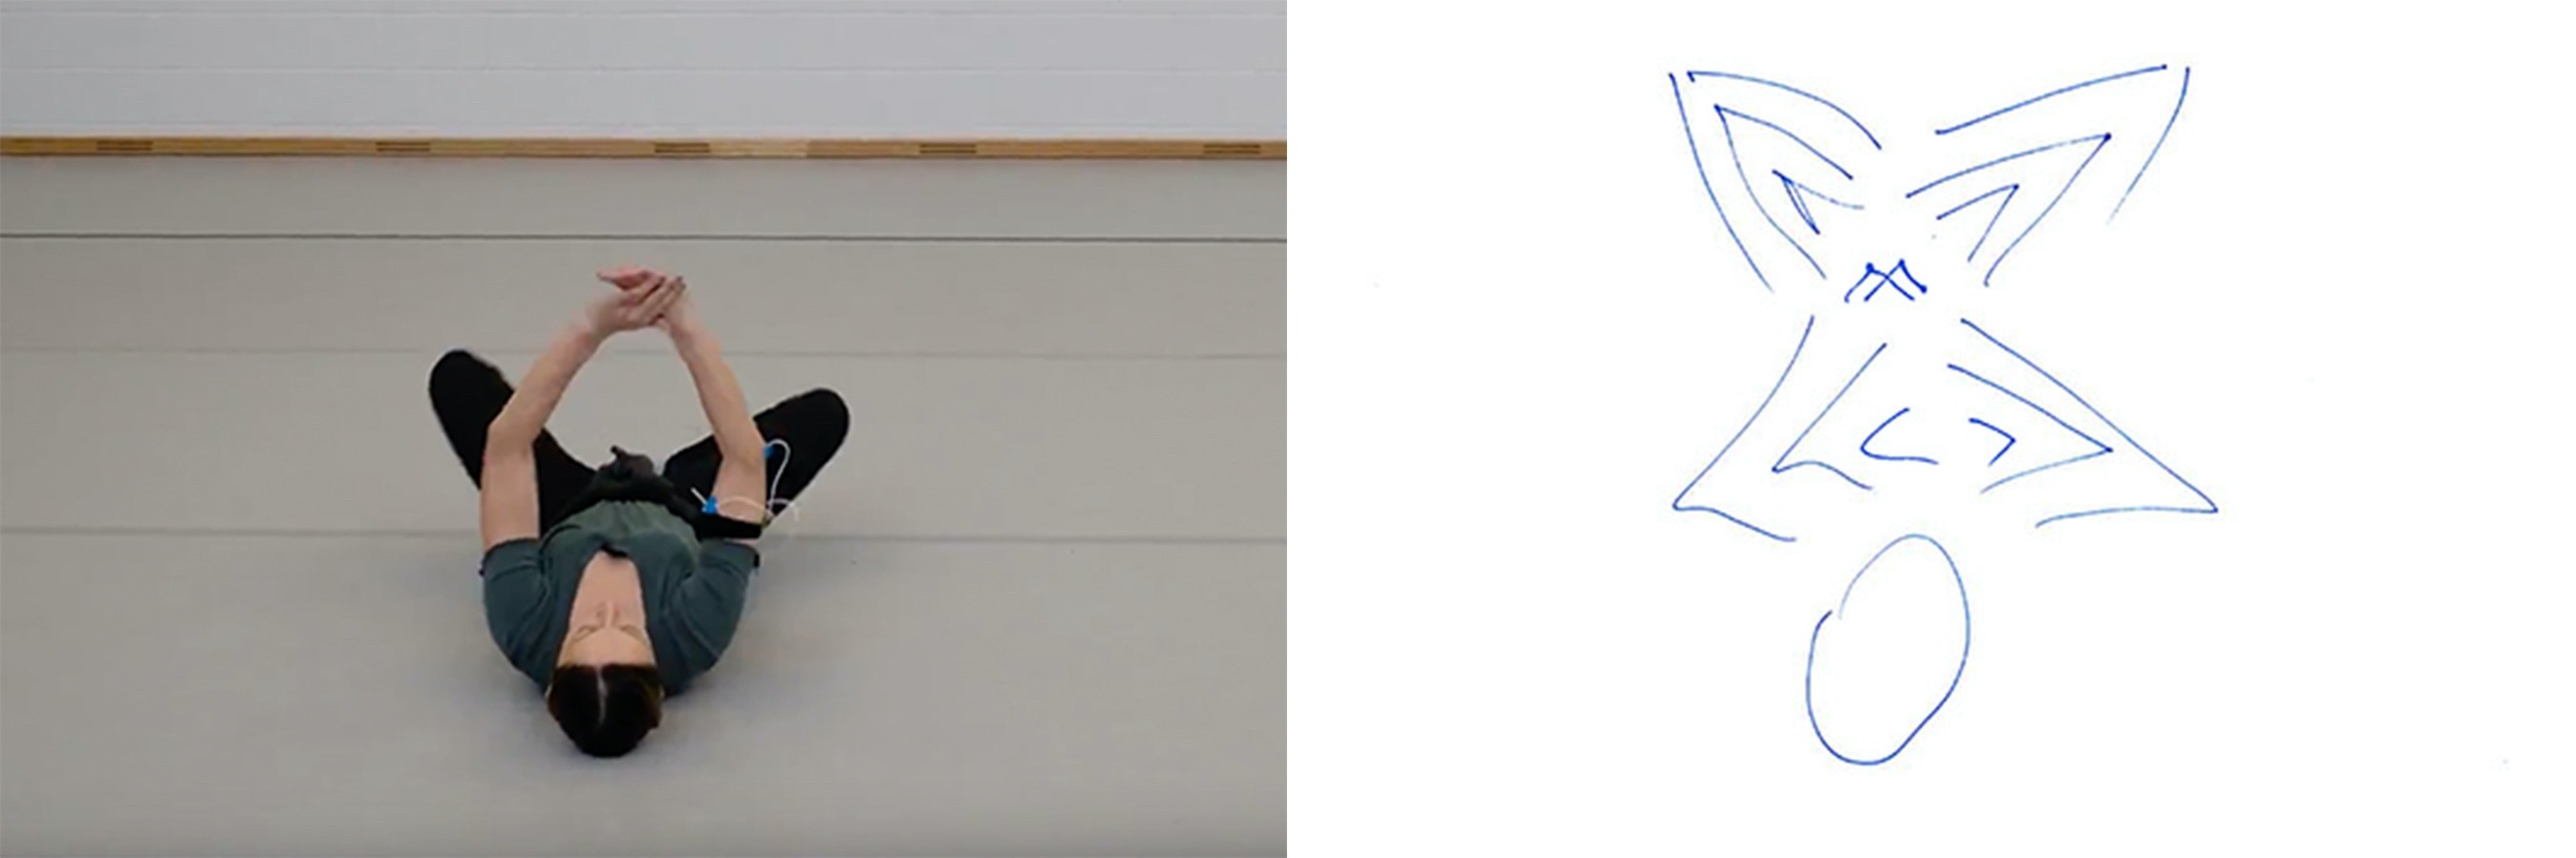
\includegraphics[width=0.9\linewidth]{Chapters/Figures/modi_dis/Zjana.jpg}
  \caption{Free-form body maps. Left: dancer executing a movement section. Right: free-form body map drawn by the same dancer corresponding to that movement section}
    \label{fig:free-form-map}
  %\Description{}
\end{figure}

The outline-based body maps (figure \ref{fig:outline-based-map})  were more constrained, and involved coloring the main body areas involved in that movement, as perceived by the participant (ten drawings per dancer – two per section of the choreography). The silhouette adopted was based on one of the outline-based body maps identified, used by  \cite{nummenmaa_bodily_2014}. Each drawing was labeled according to the specific section of the choreography that it corresponds to. A total of 150 body maps were produced (50 free-form and 100 outline-based body maps).

\begin{figure}[ht]
  \centering
  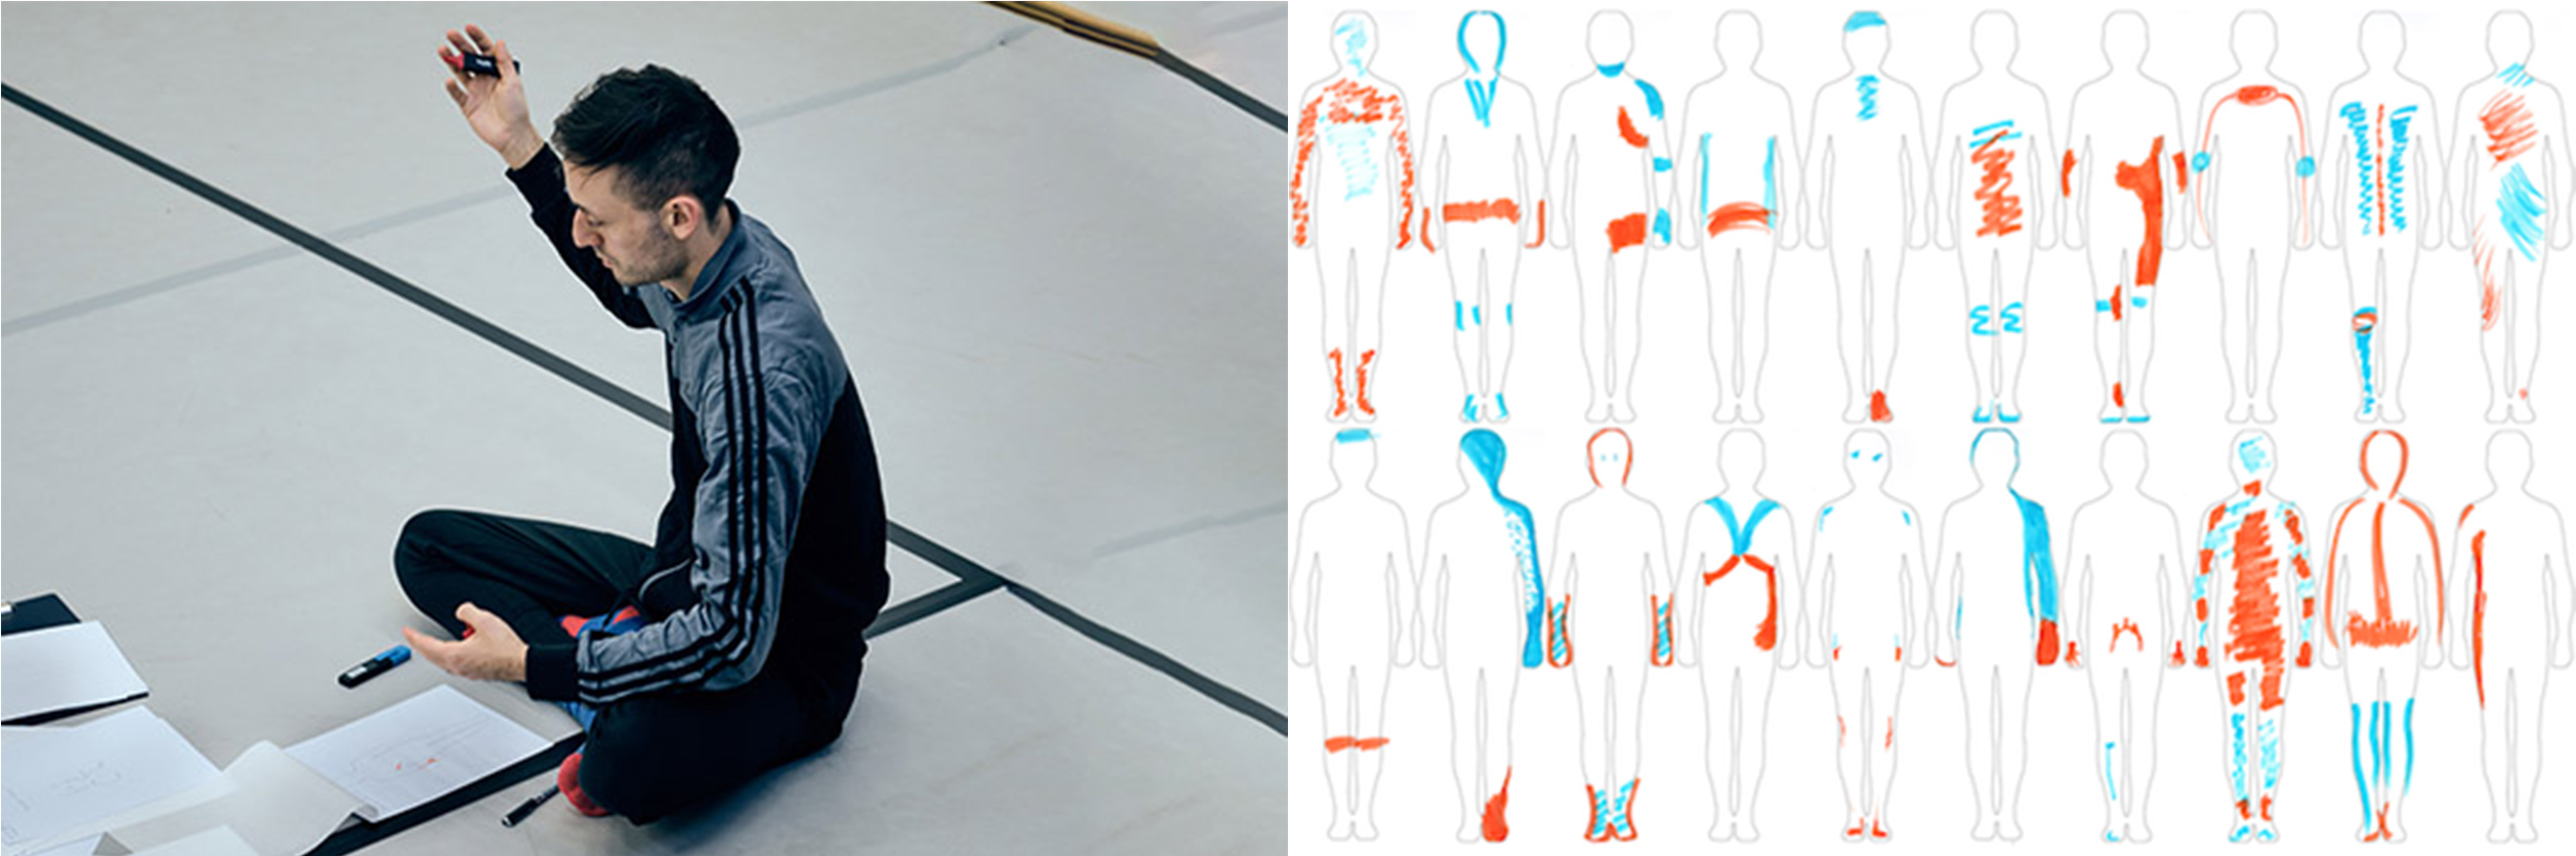
\includegraphics[width=0.9\linewidth]{Chapters/Figures/modi_dis/Juan.jpg}
  \caption{Outline-based body maps. Left: dancer partly reenacting a movement section while drawing an outline-based body map of that movement. Right: 20 of the total 100 outline-based body maps.}
    \label{fig:outline-based-map}
\end{figure}

\subsubsection{Stage 2 - Prototype development}

After the initial workshop, our research team set out to conceive approaches for interaction design and visualization, which would leverage the visual material created by dancers in Stage 1, informed by related literature. We aimed to generate motion graphics from drawings created by the performers. To fulfill that, we followed two different approaches, each considered more suited to outline-based or to free-form body maps, resulting in two prototypes.

\paragraph{Machine Learning Interactive Visuals Approach}

For the outline based body maps, we employed an approach we entitled Machine Learning Interactive Visuals (MLIV). Each body map was labeled according to a specific section of the choreography and then matched with the sensor data recorded, while the movement was being performed. We developed a MLIV system using TensorFlow (https: //www.tensorflow.org) \cite{abadi_tensorflow_2016}, capable of morphing between the performer’s body map drawings by predicting the interpolated frames, according to biosignal sensor data. The workflow is illustrated in figure \ref{fig:ml-model}. This is done through a Convolutional Autoencoder (CAE), an unsupervised model consisting of an encoder and decoder function. We adopted an autoencoder approach informed by Berman and James \cite{liapis_learning_2018}, who found that it was suited for live applications in dance. The encoder computes compressed representations of the images, assigned according to the visual features interpreted by the model, referred to as the latent vectors. To allow navigation between these vectors, the decoder is capable of generating continuous interpolations between the drawings, resulting in a series of new, reconstructed, images.

\begin{figure}[ht]
  \centering
  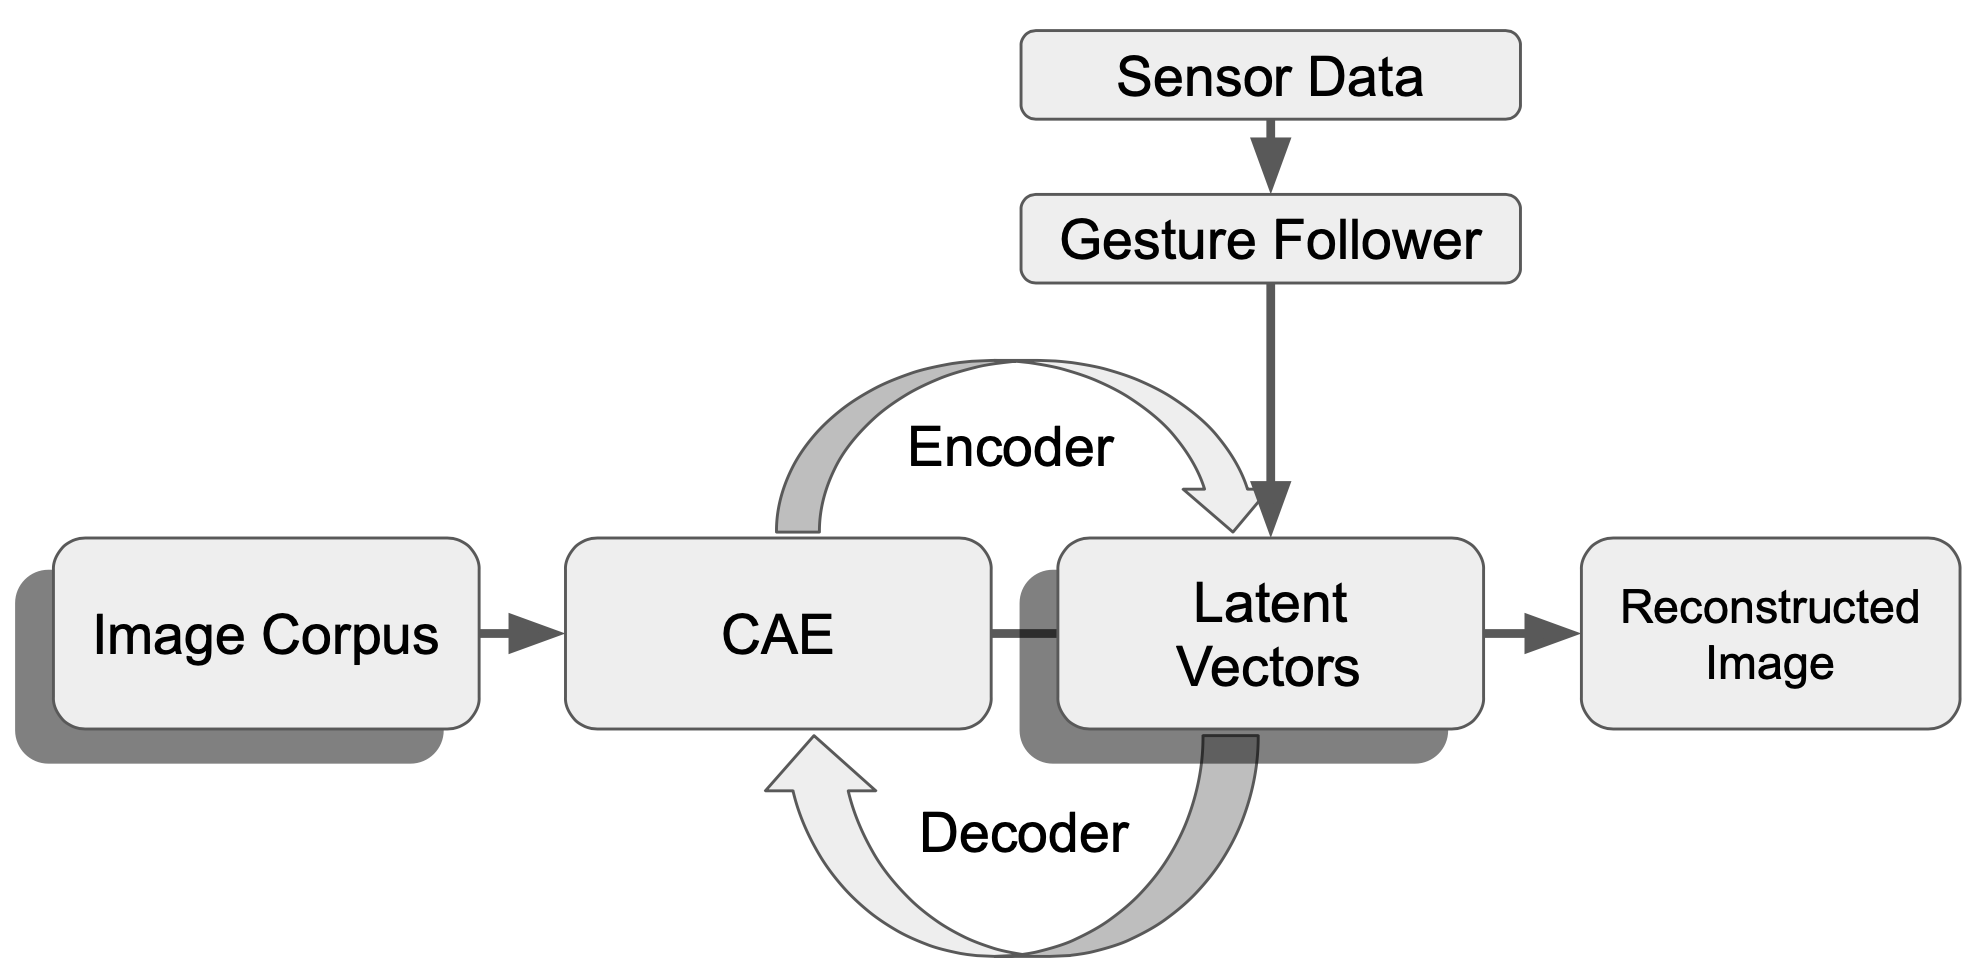
\includegraphics[width=0.9\linewidth]{Chapters/Figures/modi_dis/ml-model.png}
  \caption{MLIV design framework diagram, as followed in the respective prototype.}
    \label{fig:ml-model}
\end{figure}

To enable user interaction, we adopted a regression-based model, trained on a set of postural gestures from the performer, producing a continuous output while gestures are repeated and performed (detailed in Section X.X). We coupled the regression model with the incoming acceleration and electromyography sensor data captured from BITalino R-IoT. This orchestration allows the performers to manipulate the style and time-dynamics of the animation through movement (navigating around the latent vector space through movement).

This work led to the MLIV prototype. The system analyzes in real time the incoming sensor data from the dancer’s movement (figure \ref{fig:ml-screenshot}, first row). When fed into the gesture recognition layer, it tries to match the incoming sensor data with a segment form the pre-trained data corpus. It identifies the closest data segment match from the corpus, retrieves and adapts the body map corresponding to that movement segment (figure 5, second row). Following that, the process is repeated. When the next body map match is found, the system generates interpolated frames between the two matches (current and previous match), creating an animation (figure \ref{fig:ml-screenshot}, third row). The process then repeats again. This way, the system can generate in real time a vast number of possible animations based on the movement being executed, which would be unfeasible to generate manually.

\begin{figure}[ht]
  \centering
  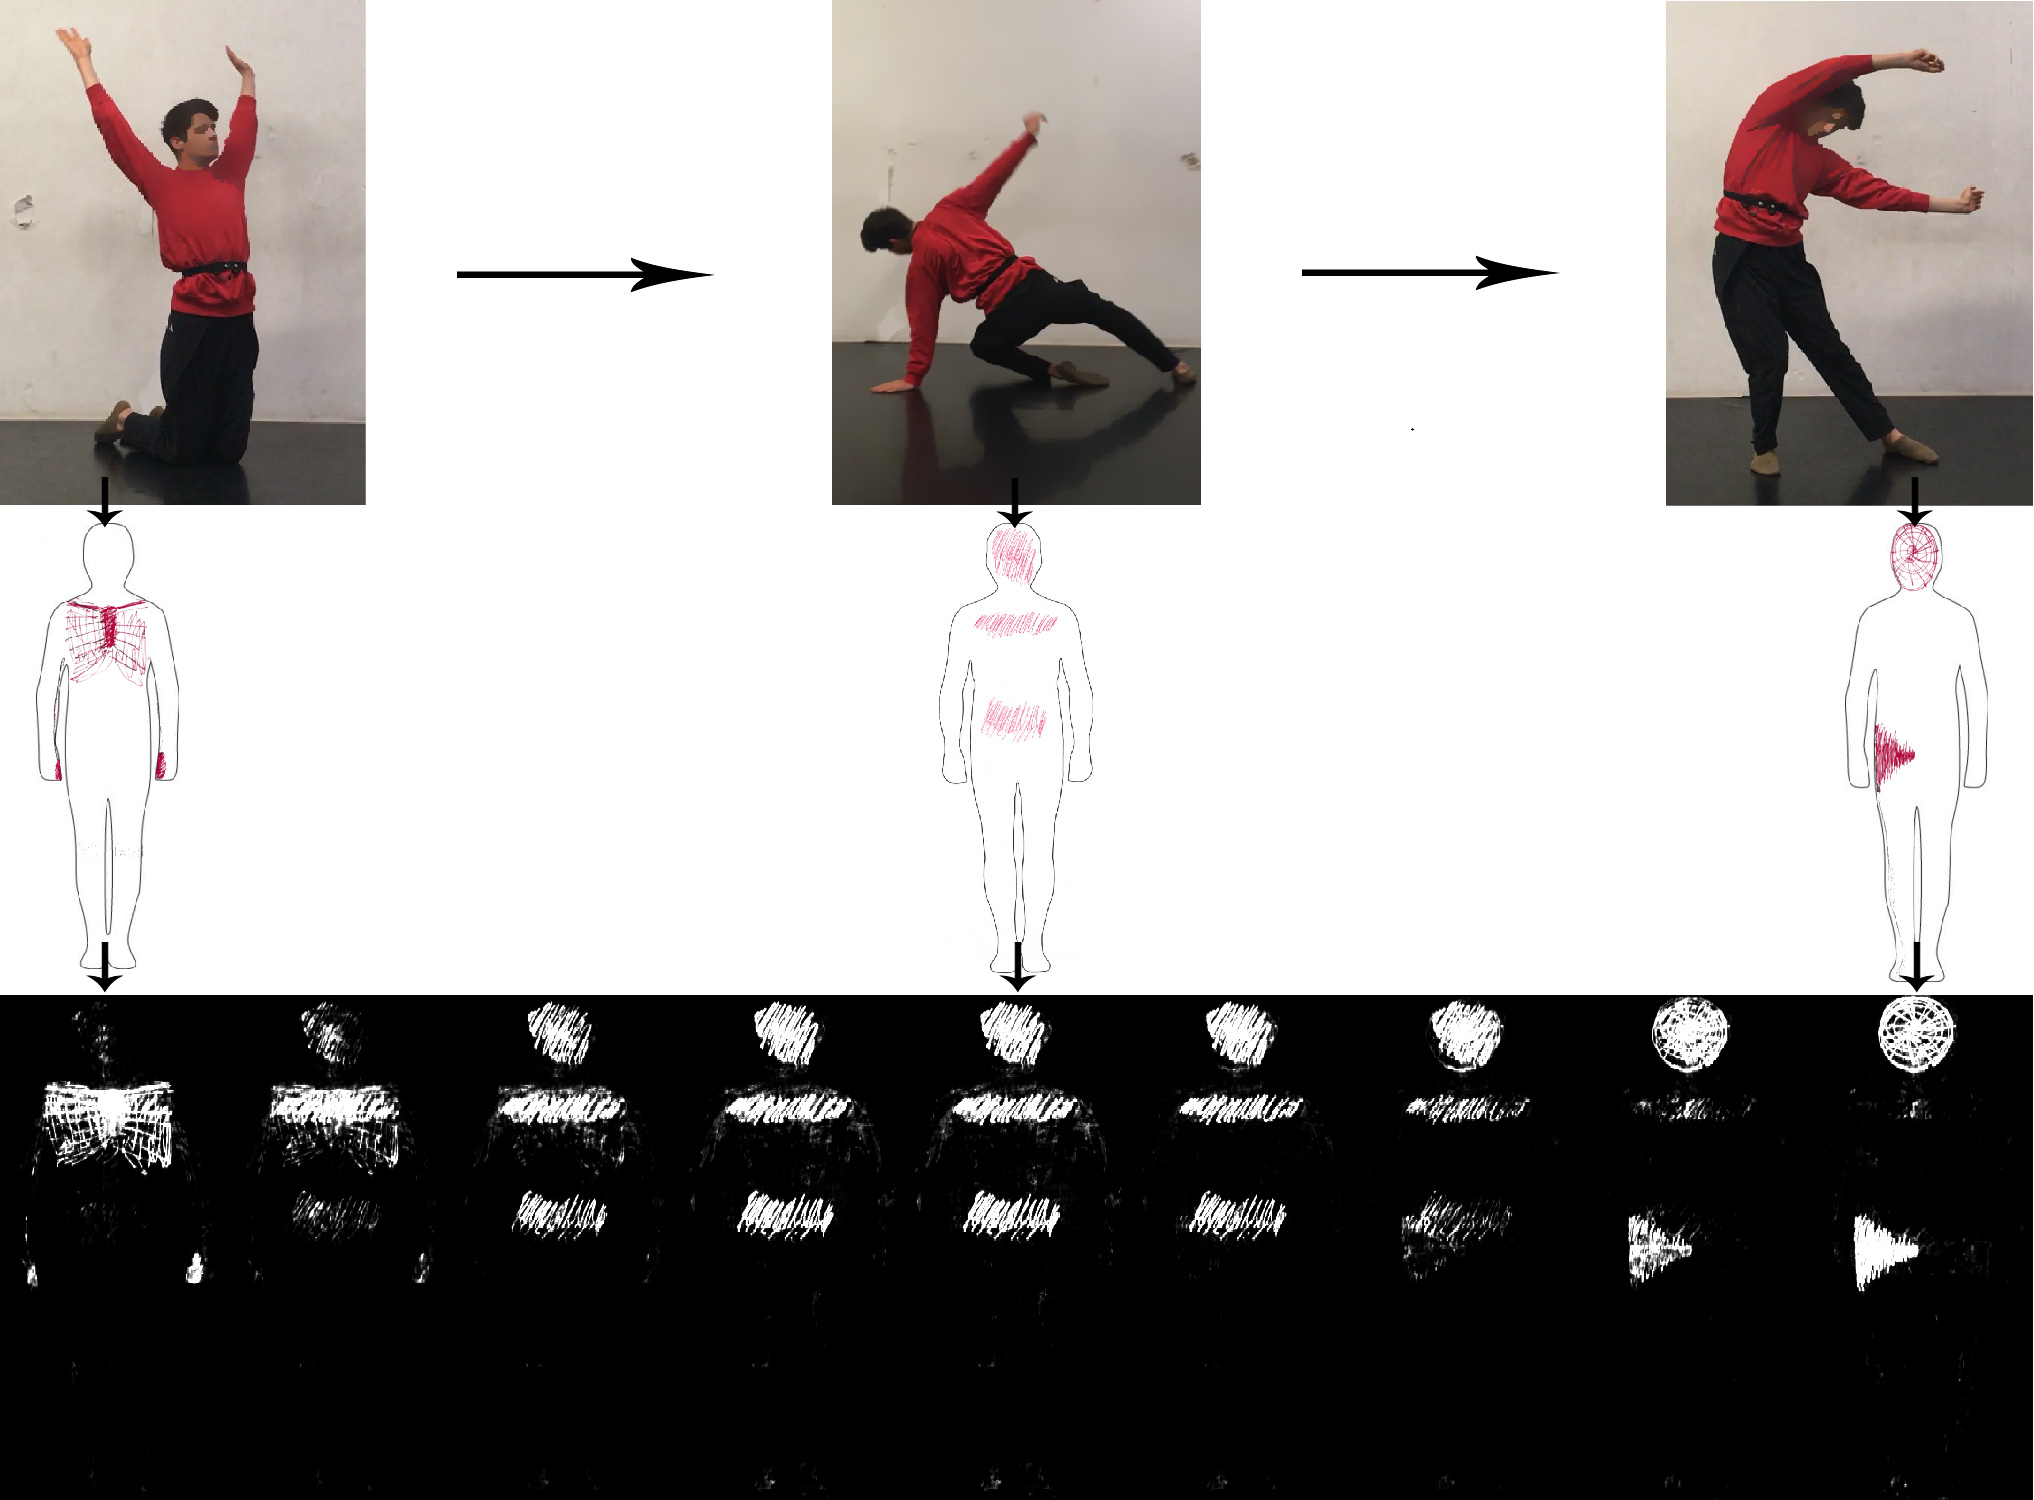
\includegraphics[width=\linewidth]{Chapters/Figures/modi_dis/sensor-drawing-3rows-large.png}
  \caption{Sequence of real time visualization frames from the MLIV prototype, based on movement and matching body maps.}
    \label{fig:ml-screenshot}
  %\Description{}
\end{figure}

% Figure Movement -Sketch - Output

% Figure 5: Sequence of real time visualization frames from the MLIV prototype, based on movement and matching body maps.

\paragraph{Composite Animation Interactive Visuals Approach}

We were aware that there would be difficulties using MLIV with the free-form body maps. Due to the relatively small number of drawings (50) and the diversity of visual features, there was a strong likelihood of overfitting – thus presuming our computational model (presented above) would not recognize meaningful patterns in the dataset. This was apparent during the initial prototyping phase, when feeding new inputs. We observed the inferred outputs would either resemble near replicas of the original data, or noisy representations, so incohernet, they held almost no association with any of the dancers’ visual intentions (i.e the original sketch).

\begin{figure}[ht]
  \centering
  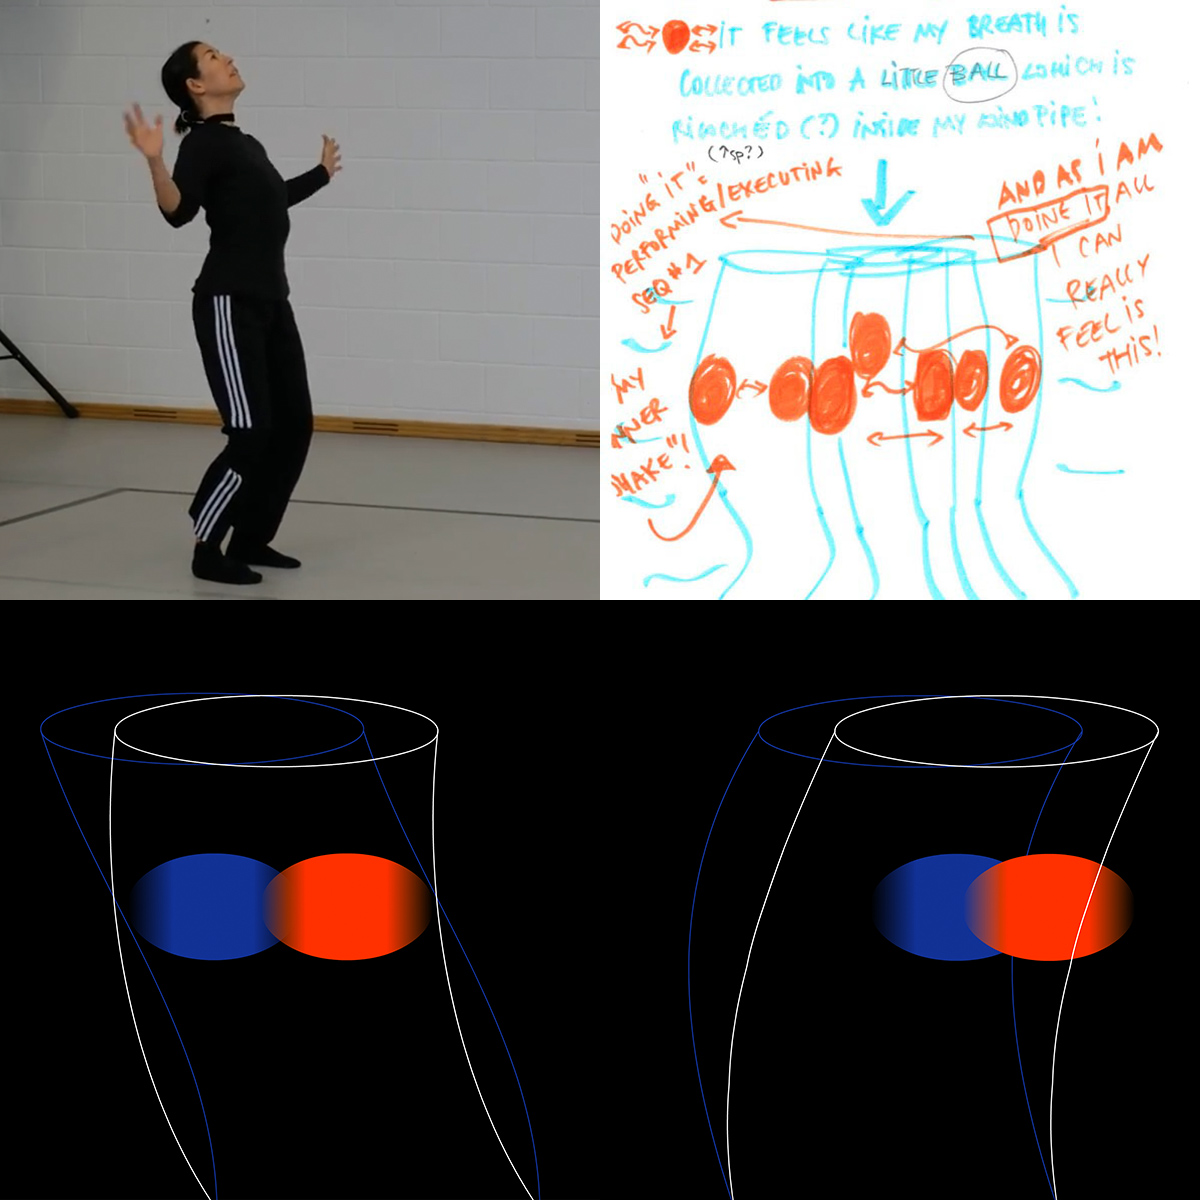
\includegraphics[width=0.65\linewidth]{Chapters/Figures/modi_dis/Stage1-animation.jpg}
  \caption{CAIV approach. Top left: dancer executing a movement section. Top right: the free-form body map drawn by the same dancer corresponding to that movement section, with annotations. Bottom: two frames of the motion graphics created by the animator, based on the documentation of the movement section, represented on top of the image.}
    \label{fig:Stage1-animation}
  %\Description{}
\end{figure}

Instead of MLIV, we adopted a ‘human learning’ approach we entitled Composite Animation Interactive Visuals (CAIV), to create interactive visuals from the free-form body maps. We use the term ‘composite animation’ to adapt the concept of composite drawings to animation. Composite drawings are used in forensic art and can be defined as freehand drawings, created by a forensic artist, combining various sources into a single graphic image \cite{stewart_forensic_2015}. These sources can be, for example, witness descriptions and CCTV footage related to a crime. To pursue this concept, we hired a professional illustrator and animator, André Carrilho, to transform the free-form body maps into motion graphics, also informed by the annotations on the body maps and the matching video sequence. With these elements, he created the different animations, in a way that respected the original body maps, while slightly simplifying and harmonizing the different animations (figure \ref{fig:Stage1-animation}). These slight simplifications and harmonizations aimed to allow for a better ‘mixing and matching’ of the animations during a performance. In this stage, the animator created ten motion graphics sequences, one per dancer (with the possibility to add more in the future) – chosen based on the potential of the respective body map for animation, while covering all five section themes. Our research team reviewed the animations as part of a ‘quality assurance’ process, to check if they conveyed the dancer’s materials well. In some cases, the animator fine-tuned the animations according to our suggestions.

\begin{figure}[ht]
  \centering
  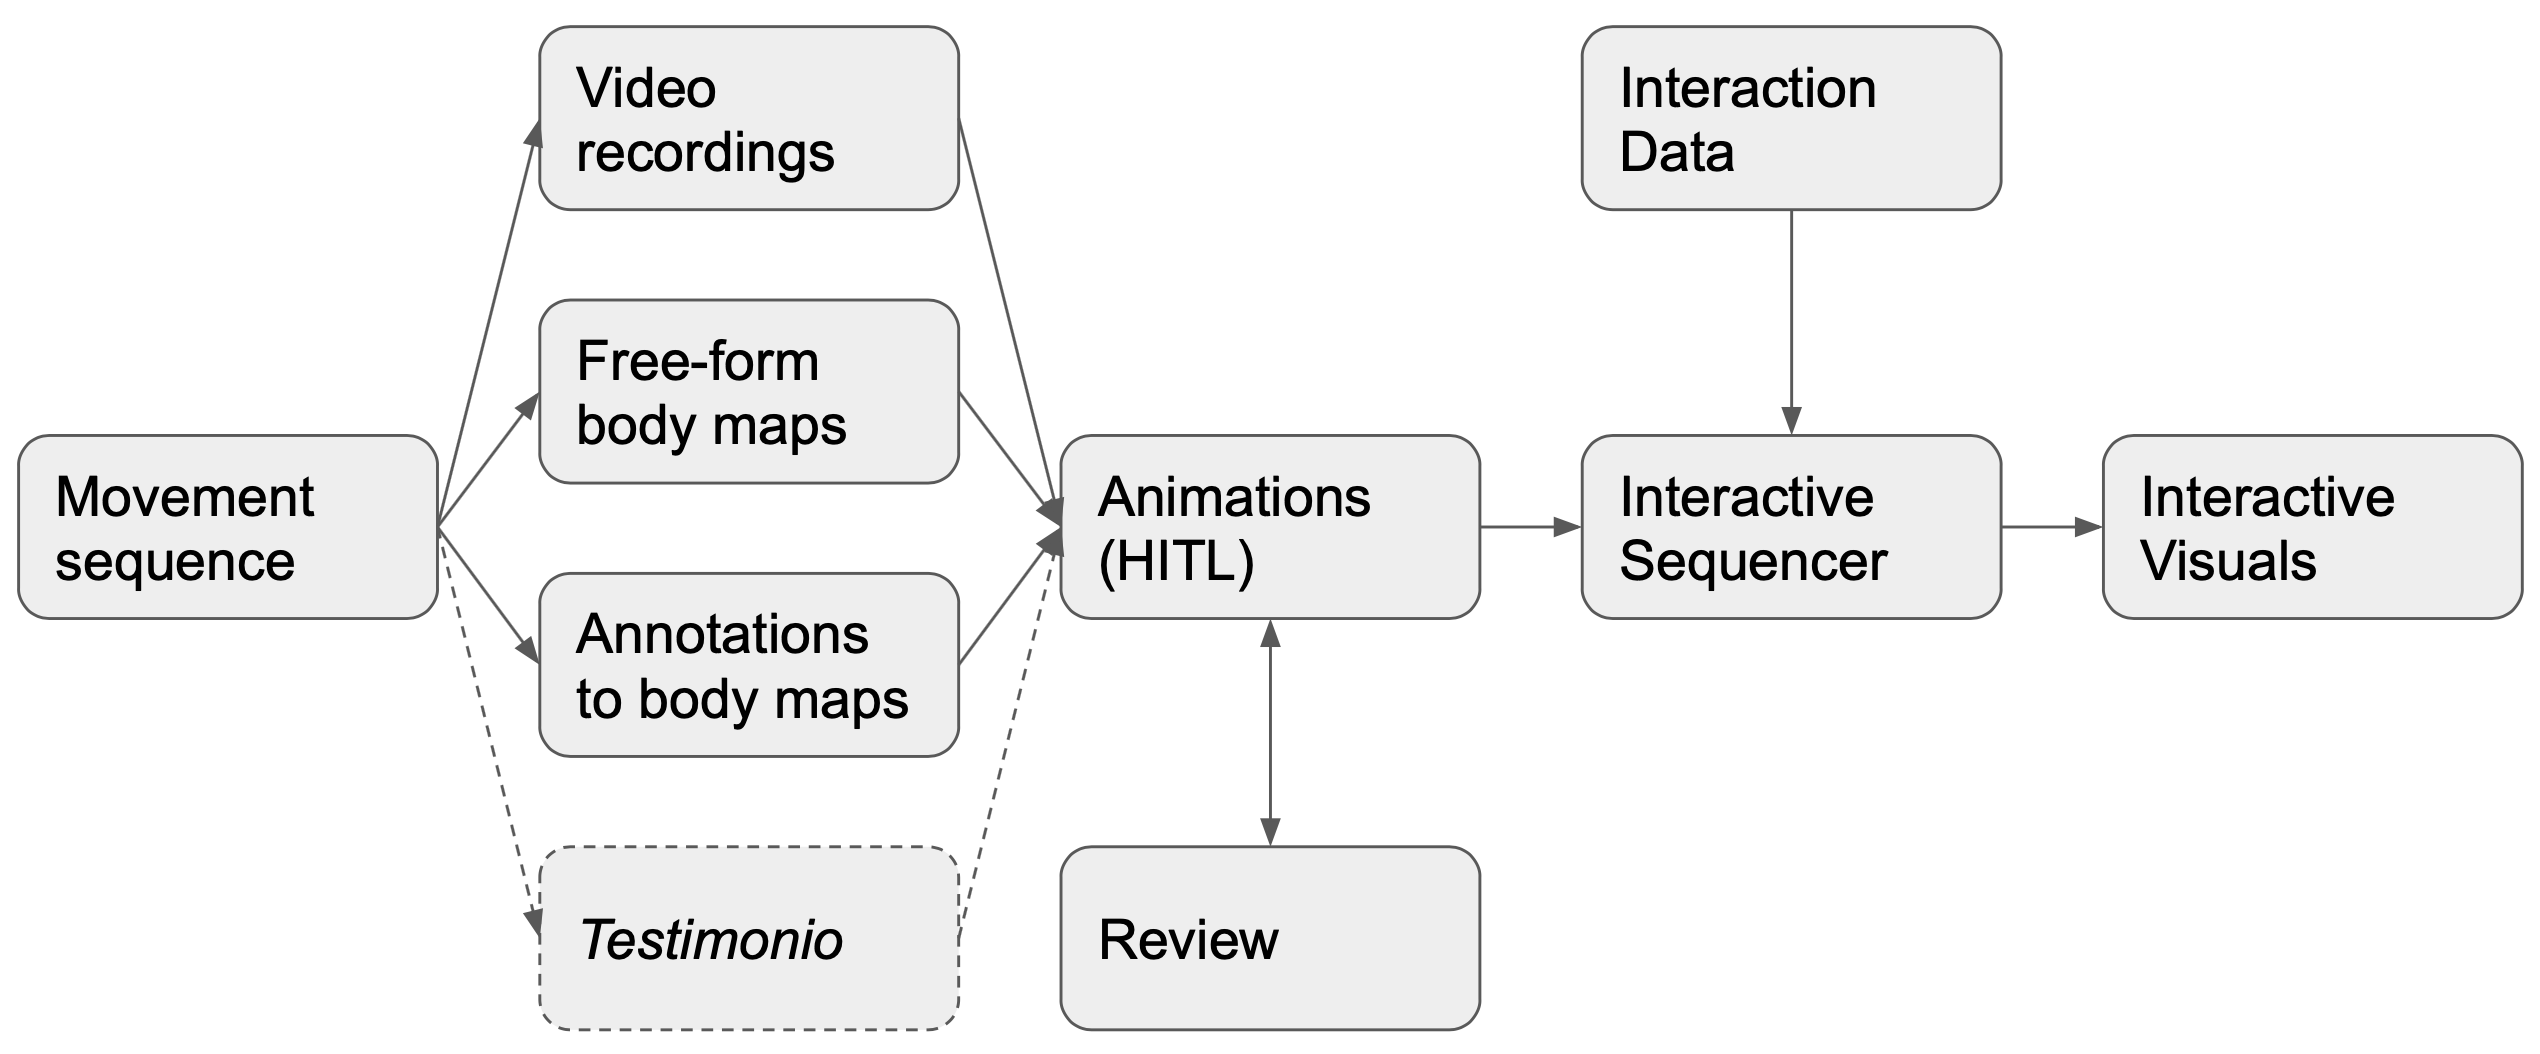
\includegraphics[width=0.7\linewidth]{Chapters/Figures/modi_dis/hitl-model.png}
  \caption{CAIV approach diagram, as followed in the respective prototype.}
    \label{fig:hitl-model}
  %\Description{}
\end{figure}

For the interaction design in our CAIV approach, we did not use ML or biosignal sensors, and focused on the non-linear sequencing of animations, in a way that would support flexible choreographic decisions. We created a visual sequencer for the animations using \textit{Isadora} (\url{https://troikatronix.com}), an “easy to use but also sophisticated software for both workshops as well as performance” \cite{delahunta_isadora_2005}. We designed a customizable Graphical User Interface (GUI) for the sequencer, to structure and trigger the animations non-linearly, onthe-fly. Figure \ref{fig:hitl-model}) shows the GUI coexistinging with video thumbnails, video preview and the data flow, allowing for spontaneous reconfiguration, while maintaining ease of use for the operator (e.g., the choreographer, the dancer or a technician).

The animations could be used, for example, as an onstage virtual ‘partner’ for the dancers (using Hsueh et al’s terminology \cite{hsueh_understanding_2019}) or as a ‘director’ (that could represent the choreographer, or another role). During the performance, it allows to display not just a single animation, but also multiple ones, as a ‘menu’ of options for the next animation (for example, visualizing the options for the next movement of a virtual entity, or the next instruction for the dancer to follow). As placeholders for animations, videos, images or text can be used. Our CAIV approach is modeled in figure \ref{fig:hitl-screenshot}.

\begin{figure}[ht]
  \centering
  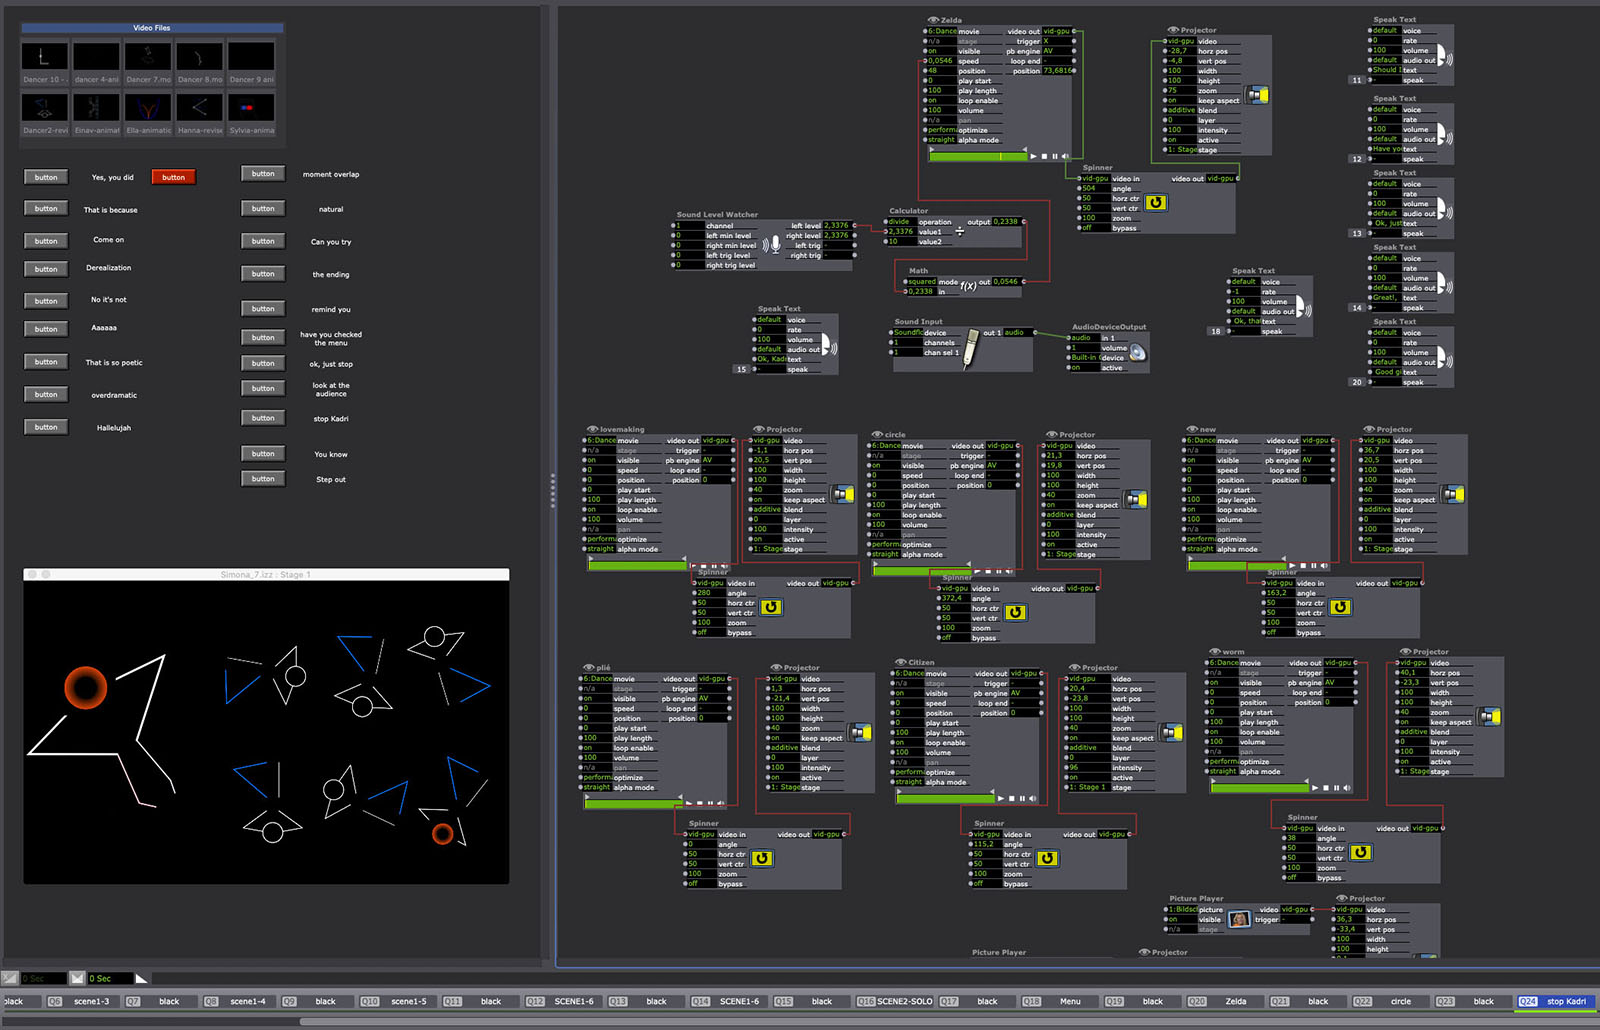
\includegraphics[width=0.65\linewidth]{Chapters/Figures/modi_dis/hitl-screenshot-s.jpg}
  \caption{CAIV prototype screenshot, as seen by the operator. Top left: animation thumbnails and GUI to trigger animations. Bottom left: preview of the visuals to be projected on stage (in this case, a image of the ‘menu’ of possible next animations in the sequence). Right: \textit{Isadora} data flow.}
    \label{fig:hitl-screenshot}
\end{figure}
% Figure 7: CAIV prototype screenshot, as seen by the opera- tor. Top left: animation thumbnails and GUI to trigger ani- mations. Bottom left: preview of the visuals to be projected on stage (in this case, a image of the ‘menu’ of possible next animations in the sequence). Right: Isadora data flow.

% Figure 8: CAIV approach diagram, as followed in the respec- tive prototype.

\subsection{Evaluation Stages}

\subsubsection{Stage 3 - Initial Evaluation Workshop and Results}

Stage 3 consisted of a four-day workshop, which took place at the Interactive Technologies Institute, Madeira, Portugal. The main objectives of this second workshop were to evaluate the prototypes and collect feedback, leading to their improvement. Ten performers attended the workshop – eight from the first event (two of the original participants could not attend), and two new performers (D5 and D10), recruited from applicants to the original call.
During the four days, the dancers freely tried out the prototypes, and gave us informal feedback, which we used to iterate on those prototypes on-the-fly. On the first day, after a general introduction to the prototypes, each participant was asked to choose one of the two prototypes, for more in-depth testing during the rest of the workshop. From then on, the dancers were organized into two groups of five participants: MLIV group, composed of D1-D5; and CAIV group, composed of D6-D10; focusing on the respective prototypes (figure \ref{fig:tests}). On the last day, we organized two focus groups (one with each group of participants), aiming to give feedback to the respective prototype. In the focus group sessions, participants were asked to convey their impressions of the prototypes, and were prompted to mention positive and negative aspects. The two sessions had a duration of approximately one hour each. The transcriptions of the two focus groups were subjected to thematic analysis (as presented in the Methods section), resulting in four common themes: introspective visualization; affordances as inspiration and instructor; communication with audience; and openness and modularity.

\begin{figure}[ht]
  \centering
\hspace{8em}
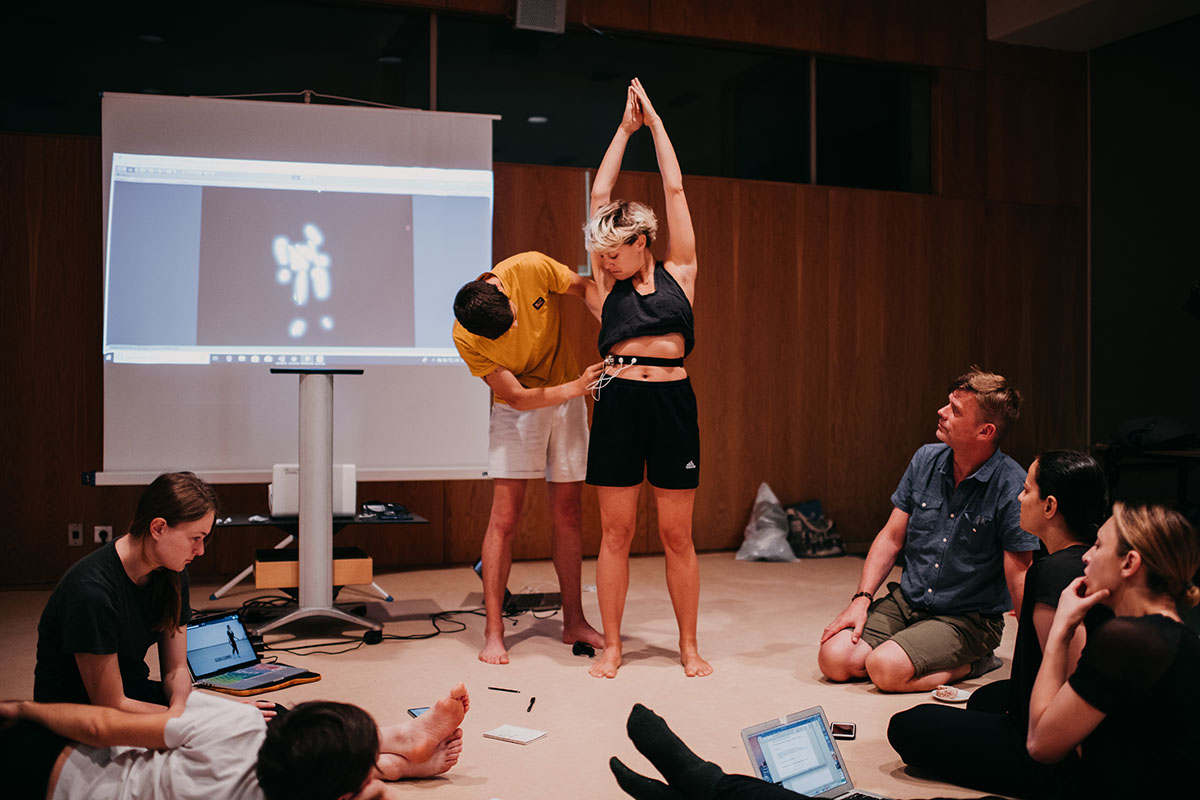
\includegraphics[width=0.7\linewidth]{Chapters/Figures/modi_dis/ml-test-s.jpg}
\hspace{-12em}
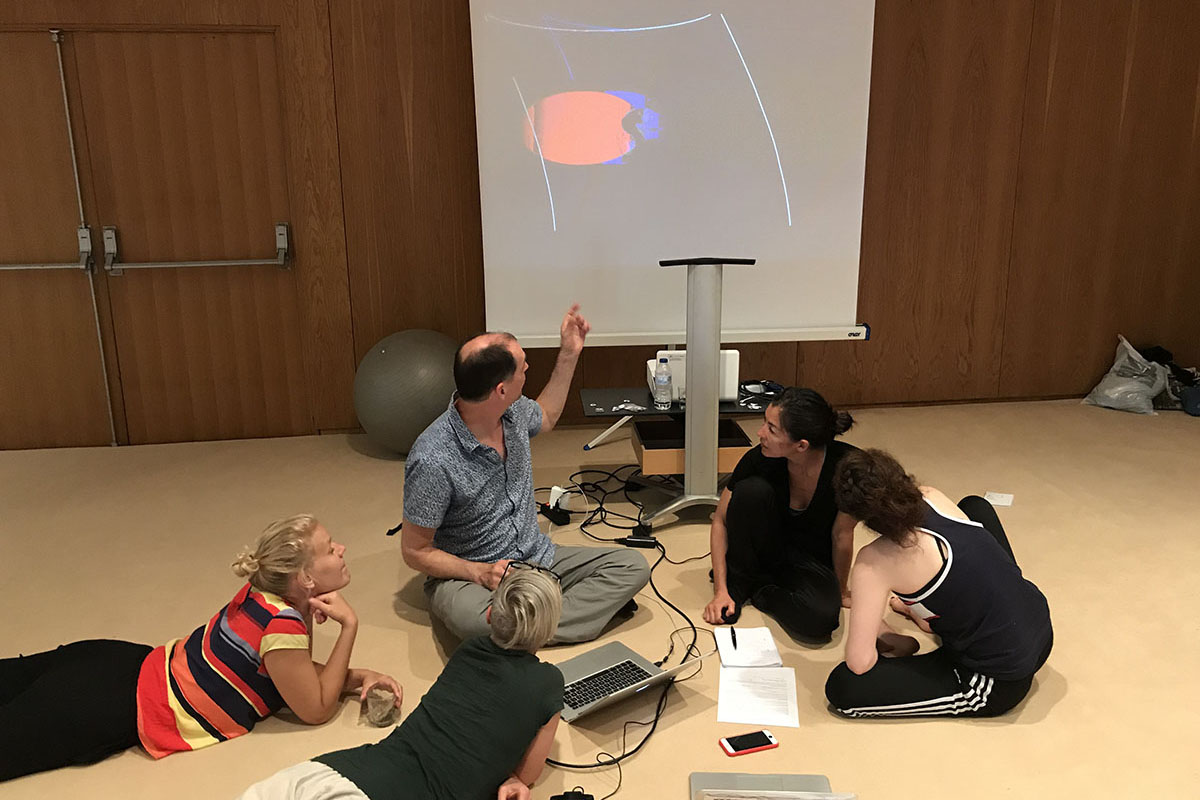
\includegraphics[width=0.7\linewidth]{Chapters/Figures/modi_dis/hitl-test-s.jpeg}
\caption{Initial prototype evaluation. Top: MLIV group. Bottom: CAIV group.}
\label{fig:tests}
\end{figure}

% Figure 9: Initial prototype evaluation. Left: MLIV group. Right: CAIV group.

\paragraph{Introspective Visualisation.}

\textbf{MLIV group:} All participants mentioned they appreciated the capability of the MLIV prototype to visualize the subjective and introspective aspects of the body, as exemplified in the following statements:

\begin{center}
\begin{tabular}{ p{13cm}}
\textit{It takes your internal experience, this subjectively live body experience and puts it outside. (D1)
[The researchers] included our initial perspectives in order to develop this prototype, not just the movement, not just the shapes of movement, but also the introspective aspect of how you feel concerning movement. (D2)}
\end{tabular}
\end{center}

Although some participants enjoyed that the MLIV prototype took their sketches as a starting point: “It provokes the imagery according to our own notation” (D2), others considered the visuals monotonous (D3, D5). \textcolor{red}{include quote also}

\begin{center}
\begin{tabular}{ p{13cm}}
\textit{it was already like this anthropomorphic thing was very dominant already from the exercise there. And I agree, for me it was a very... the aesthetic of this output and the human form, for me it was very limiting while using it}
\end{tabular}
\end{center}

\textbf{CAIV group:} D9 enjoyed the capability to visualize the dancer’s decision process in the CAIV prototype: “We are revealing things that happened in the dancer’s head while we are dancing (...) to reveal this process that we are doing, actually most of the time unconsciously. Deciding. What is next? ”

\paragraph{Affordances as Inspiration and Instructor.}

\textbf{MLIV group:} Participants enjoyed the bodily data affordances of the MLIV prototype (D1, D3, D4), which changed their behavior: “It puts me in a state of not doing form, because it’s not a camera, but it puts me in a state of exploring, like, weird internal stuff that I don’t usually do” (D3). All participants considered using sensors to be inspiring for movement. As D2 stated: “It opens a lot my imagination of how to interact with a system, and what the system reads in me, and what it incorporates in my somehow subjective feelings toward my own movements”. Participants mostly disliked the slow reactivity of the MLIV prototype (D2, D5), although this was considered adequate by D1: “it takes a bit of time to see, which is how I deal with my dance practice”.

\textbf{CAIV group:} The dancers valued the non-linear flow of the CAIV prototype. A possible scenario that was identified is the system providing instructions to the dancer: “I think of a live situation where the dancer is kind of a slave of this big king of dance who’s sending me here and there. And I think it could be interesting because the performance would be different every time” (D10). Two dancers (D6 and D10) suggest using randomness to select the next steps in the sequence, instead of an interactive selection.
5.1.3 Communication with Audience. 

\textbf{MLIV group:} Participants recognized potential for communication between dancer and audience in the MLIV prototype: “I can make it clear enough the relationship between my movement and what the audience sees” (D2).

\textbf{CAIV group:} D7 identified potential in the CAIV prototype to make the audience move, using the system to output instructions for that movement. Related to this logic, D6 identifies pedagogical potential in the prototype, as a teaching and learning dance tool, suggesting adapting it to an interactive installation.

\paragraph{Openness and Modularity. }

\textbf{MLIV group: }D2 felt involved in the co-design process of creating the MLIV prototype: “It’s also a tool that we somehow coded, like participating in the process of coding”. Dancers wished to combine the prototype with motion capture (D2) and other types of sensors (D1). The wish for modularity was summarized by D4: “I am also more interested in trying out different possibilities, what are the possibilities where I can take the input from, which are the possibilities for the output” (an opinion echoed by D3).

\textbf{CAIV group:} The CAIV prototype showed potential as a tool to build choreography (D6, D7, D9), characterized as: “An open structure, which can be put down and rebuilt in a different way” (D9). However, it can be laborious, due to the need to prepare visual materials (D7, D10). Participants wished for a modular structure for it, combining features and functionalities taken from the MLIV prototype, such as: to add sensors (D7, D9) or ML (D7, D10)

\subsubsection{Stage 4 - Rehearsals of Choreographies and Evaluation Results}

After the Stage 3 workshop, participants could submit proposals for choreographies to be developed in the scope of [anonymized project]. Eight participants in the previous workshops submitted proposals, and four were chosen by the research team, based on the quality of the artistic concept, innovative approach and feasibility. Two of the selected proposals included the use of the MLIV and CAIV prototypes. For the scope of this paper, we focus on the work developing the two respective choreographies. The two participants (authors of the proposals) will now be referred to as ‘choreographers’, to reflect their change of role. The choreographer using MLIV will be referred to as C1, and the one using CAIV will be referred to as C2.  

C1’s proposal text was aligned with our aim of exposing non-visible elements:

\begin{center}
\begin{tabular}{ p{13cm}}
    \textit{In augmenting the interior realities through explorations of imaginary, sensations, creative fantasy, and the inner body-textures of the dancers relative to the exterior world (spectator), I seek to demonstrate unusual characteristics of dancing by creating a (visual) menu consisting of unusual perspectives of a dancing Body}
\end{tabular}
\end{center}

C2’s proposal was equally in line with our aim, focusing on the thinking and choice processes of the dance artist. It stated:

\begin{center} 
\begin{tabular}{ p{13cm}}
    \textit{I want to give the audience an insight on dance making, by showing the invisible process behind the choices one makes when creating a piece. (...) The audience will perceive 2 types of presentations: a human one and a virtual one. (…) Its proposals [of the virtual entity] would materialize in Animated Drawing, that envision its own movements, accompanied by related poetical explanations.}
\end{tabular}
\end{center}

Meanwhile, we made improvements to the prototypes, to address limitations identified in Stage 3. In the MLIV prototype, we introduced the wearable form-factor for the \textit{BITalino R-IoT}, with the sensory components embedded into a wearable enclosure; this reduced the noise in the signal during rapid movements, while allowing for faster setup times. In the CAIV prototype, we added new GUI elements in \textit{Isadora} for ease of operation, this fine-tuning of the GUI continued also during the residency according to the needs of C2. The animator was commissioned to develop ten more composite animations, defined with C2.

In Stage 4, we organized a 12-day artistic residency with the selected participants. The residency took place in the [anonymized] performance space. The objective was to develop each choreography and rehearse it, while continuously evaluating and fine-tuning the respective prototypes. It was intended to be more in-depth than previous workshops: it had fewer participants, and a longer duration, suitable for the rehearsal of a short choreography, building upon previous work. Choreographers were given the chance to work with local dancers (C1 chose two dancers, and C2 picked one). 

We arranged six separate six-hour studio sessions with each choreographer, across the 12 days, in alternating days (figure \ref{fig:rehearsals}). At the end of each session, we conducted short semi-structured interviews (six in total for each choreographer). We asked questions related to the use of interactive and visualization technology and the development of the respective project. The transcriptions of the interviews were subjected to thematic analysis (as presented in the Methods section), resulting in three common themes (body visualization aesthetics; feedback loops and connections; workflow and workarounds).  

\begin{figure}[ht]
  \centering
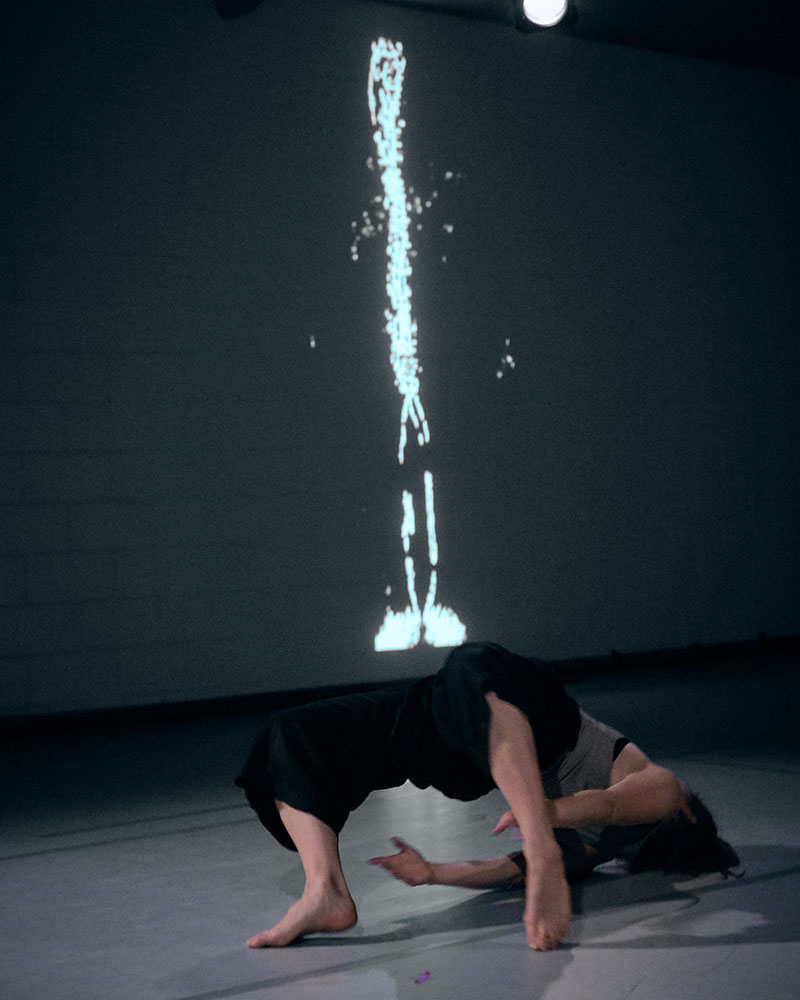
\includegraphics[width=0.475\linewidth]{Chapters/Figures/modi_dis/Sylvia.jpg}
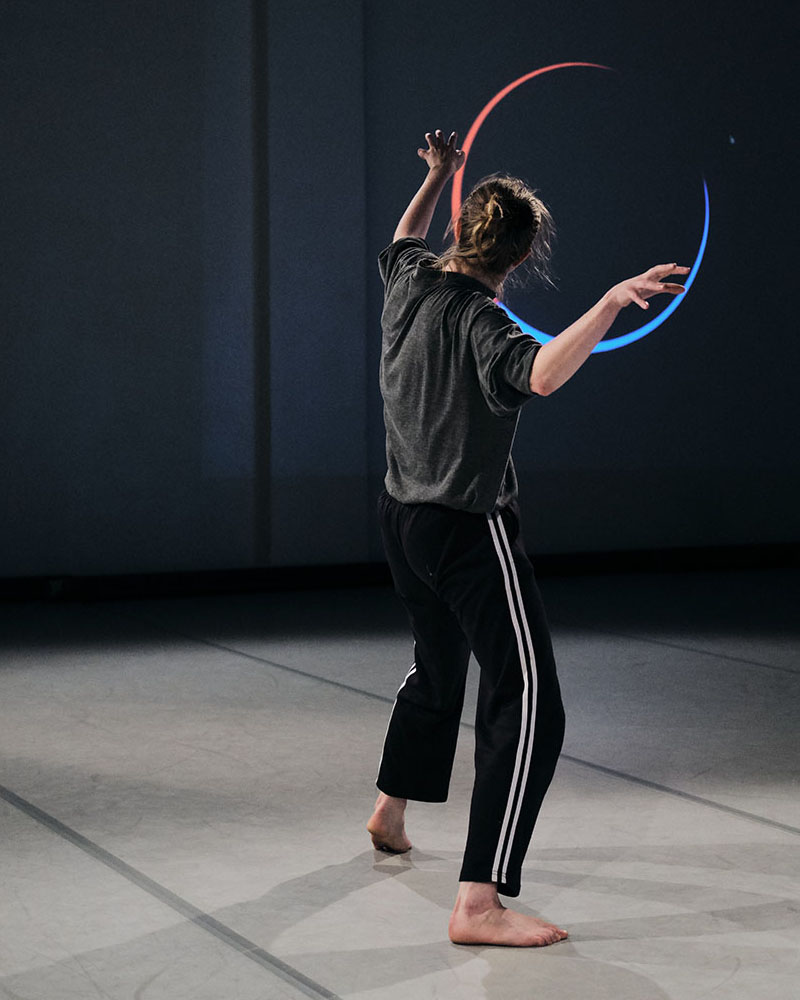
\includegraphics[width=0.475\linewidth]{Chapters/Figures/modi_dis/Kadri.jpg}
\caption{Images from the residency rehearsals. Left: MLIV approach. Right: CAIV approach.}
\label{fig:rehearsals}
%\Description{}
\end{figure}

\subsubsection{Body Visualization Aesthetics}

C1 enjoyed how the MLIV prototype facilitated visualizing biosignal data: “\textit{It's nice to be able to  see how biological information through the human body can affect or create [visual] effects}” (day 1). In particular, she felt that its pulsating aesthetics  highlighted the physiological side of the dancer: “\textit{It gives the breathing element. It shows the humans a little bit more delicate. It simulates organs, the idea of breath}” (day 3).

C2 used the animations in the CAIV prototype to simulate an artificial entity: “\textit{This visual means the body of another entity in a way}” (day 4). She enjoyed the minimal animations, representing the body of this entity: “\textit{I like [anonymized animator’s] drawing very much, I think we will get to a very beautiful action, a minimal kind of body}” (day 6).

\subsubsection{Feedback Loops and Connections}

C1 used the MLIV prototype to create a feedback loop between dancer and visuals, where the dancer influenced the visuals through the sensors, and the projected visuals in turn influenced the dancer: “\textit{a looping system, biological, digital, back to biology}” (day 1). To find that feedback loop, she explored different movements and system settings, “\textit{Trying to find the right kind of feedback that can trigger a movement or generate movement that's still justifiable in contemporary dance}” (day 1). By day 4, she felt “\textit{It did generate new movement, at least new possibilities for movement}”.

C2 wished to have a “\textit{dialogue}” with the dancer, by interacting herself with the visuals, through the CAIV prototype (day 1). With this system, she felt that she is connecting visuals and dancer: “\textit{I'm creating connections between image and body}” (day 4). By the end of the residency (day 6), she felt that the operator role is very efficient: “\textit{I liked that I could interact with [the dancer] in real time}”.

\subsubsection{Workflow and Workarounds}

C1 recorded and edited a large number of visuals generated during rehearsals, which she used to create a balance with interactive moments that she could not control, due to slow responsiveness of the MLIV prototype: “The film was something I could control, which was a nice balance with everything i could not control. Which was the live situation” (day 6).

C2 considered that the CAIV prototype was a quick tool in setting up the animations and visuals in the software, despite the laborious aspect of the prototype identified in Stage 3: 
“\textit{I think it's very good to work like this, really have a software that helps you create this structure, because it's about scoring and structuring in real time, and being able to make modifications in real time}” (day 3). On the final day (day 6) of the residency, in reference to our system, C2 stated “\textit{I have discovered this very efficient tool of structuring material very very fast}”. This allowed C2 to overcome the short time for developing the choreography: “Five days is not a good time for research. Meaning we need more time” (day 6, last day, in reference to the five previous days).

\subsection{Discussion}

We developed two design approaches to create interactive visuals for dance, based on machine learning and composite animations (MLIV and CAIV). Both rely on body maps drawn by dancers, based on their somaesthetic impressions. We first discuss aspects related to each of our two approaches, and then more generic aspects.

\subsubsection{Organic and Introspective Interactive Visuals, Machine Learning Approach}

The MLIV prototype was considered successful as a tool for revealing internal bodily processes, by the five dancers that evaluated it in Stage 3. Dancers appreciated that visuals took their own “notation” (D2) from their body maps as a starting point. C1 used the system for a longer time in Stage 4, and described the aesthetics of the system in more detail, showing a deeper understanding of its design, namely its organic and breathing-like visual affordances. On the interaction side, dancers in Stage 3 highlighted the impact that the system had in their own movement and even in their imagination (D2). In Stage 4, C1 explored this to create a feedback “looping system” between the biological, the digital, and back to the biological. She felt she achieved “new possibilities for movement”. We believe our MLIV approach complements related ML and movement approaches, such as \cite{murray-browne_latent_2021,silang_maranan_designing_2014}. These focus on other aspects of the movement data (flexible mapping and data classification), while our system focuses on visualization of inner aspects of the body.

\subsubsection{Accounting for Slow Responsiveness in Latent Steps}

The MLIV prototype had limitations in terms of responsiveness, which can be attributed to a small corpus of body maps (only 100) and limited sensor data collected. We applied a low-pass filter to the frame interpolation layer to compensate for identified abrupt jitters. However, this resulted in slower reactivity, both in terms of latency and slowness of the visualisation, relatively to the corresponding movements. This slow reactivity was considered by some dancers to be problematic in account of their first impression taken during Stage 3. To mitigate the risks of a slow responsiveness of the system in a performance, C1 combined real time visuals from the MLIV prototype with pre-recorded videos of visuals from rehearsals. We hypothesise that adding more drawings to the corpus, and collecting more matching data from the moment (potentially, with added sensors) could improve this responsiveness.

\subsubsection{Connecting Idiosyncratic Visuals with Movement, Composite Animation Approach}

Due to the more idiosyncratic nature of the free-form body maps, a different approach based on composite animations was pursued. To add interactivity to the resulting animations, we developed a dedicated system with Isadora, the CAIV prototype. The resulting animations were considered aesthetically successful by C2, and she enjoyed their minimalism. She used the animations to represent the body of an artificial entity that would enter a dialogue with the dancer. C2 controlled this artificial entity herself, by operating the CAIV prototype. This way, she could interact with the dancer in real time, which she enjoyed. The animations, grounded on dancers’ movement and related somaesthetic impressions, together with the sequencing system, allowed her “creating connections between image and body” (C2). The sequencing system for the animations was also considered successful in terms of visualizing inner processes. This relates to the proposal of revealing a movement decision process realized in our preliminary focus group \cite{masu_how_2019}. In the initial evaluation, D9 stated that the CAIV prototype had the potential for “revealing things that happened in the dancer’s head while we are dancing”, the decision process of what movement to execute next. This logic was implemented by C2 in Stage 4 by showing a ‘menu’ of animations that could come next, and then triggering one of them.

\subsubsection{Comparing Visualization Approaches}

We now compare the two adopted approaches for revealing the inner processes of the dancers. We argue that an MLIV approach can be beneficial with more constrained body maps – such as the outline-based ones, with specific rules for drawing, as we have used. In our case, coloring specific areas of the body according to a certain criteria – parts of the body involved in a movement. These constraints are beneficial for training an ML system, especially when having access only to a relatively small corpus of drawings.

A CAIV approach can be preferable when the body maps are more freeform, where the visual qualities are harder to represent with a computational model. This CAIV method is clearly more laborious, as there is a need for manually generating animations. It also requires a system for adding interactivity to trigger the individual animations (such as our CAIV prototype), rather than a continuous morphing of the visuals, in the way that MLIV allows.

We are aware that forcing a choice upon participants between constrained and free-form body maps creates a “conceptual dichotomy” that should be avoided in soma design, as stated by Höök et al. \cite{hook_soma_2019}. Our participants were dancers, hence “somatic connaisseurs” \cite{schiphorst_self-evidence_2011} and fluent in expressing their impressions in both types of body maps. But other participants may not be as comfortable expressing their somatic experiences with both. Therefore, it is useful to have the option to use either MLIV or CAIV, or both, depending on the preference of dance artists. Eventually, a future hybrid solution could also be developed, combining both approaches.

Recent literature in embodied interaction has focused on the importance of accounting for “non-normative bodies” \cite{spiel_bodies_2021}. We believe that our MLIV approach has a potential for this, due to its flexibility of mappings – it is not a ‘one size fits all’ solution and can be adapted to a wide range of bodies. However, it relies on constrained, outline-based, body maps. These may suggest a ‘body norm’, which is undesirable. The free-form body maps are more inclusive in terms of body representation, as they allow for an entirely individual approach. This points once again for the potential of a hybrid solution, merging the flexible mappings of MLIV and the idiosyncratic representation of free-form body maps.

\subsubsection{Non-human Engagement in Hybrid Virtual Environments}

Using a multistage co-design process facilitated that the systems developed for interactive visuals respected the vision by the participants, from the early sketches until the final rehearsals. Throughout our study, other perspectives have emerged. Our participants identified other actors and use cases that could benefit from our visualization approaches. In particular, this emerged in Stages 3 and 4, when our participants could use and explore the artifacts created. In \textbf{Stage 3}, the focus was mainly on testing, and therefore on the use. Different possible uses and contexts of use were suggested by participants based on their reinterpretation of the artifacts. In line with our design aim, dancers identified potential for enhancing the communication between the dancer and the audience, in both prototypes (D2, D7). However, three further possible uses for the CAIV prototype were also identified: as an audience interaction tool (D7); as a dance pedagogy tool (D6); and as a choreography creation tool (D6, D7, D9). This positions the artifacts beyond the originally intended category of augmented performance and into the categories of education and choreographic tools, according to the taxonomy in \cite{raheb_dance_2019}.

\cite{dix_designing_2007}. During this artistic residency, indeed, C2 highlighted the potential of the CAIV prototype to be both a virtual ‘partner’ for the dancer \cite{hsueh_understanding_2019} and a mediator between choreographer and dancer. This situates the system (as used by C2) in the category of agent collaboration, in the taxonomy by Zhou et al. \cite{zhou_dance_2021}. This observation was not only a \textit{reinterpretation} of the system, but actually lead to the fine-tuning of the design, \textit{adapting} the GUI, to facilitate the role of C2 as an operator in dialogue with the dancer. C1 also appropriated the artifact to create a feedback loop between the visuals and the dancer, introducing further adaptations, as different movements were tested in combination with adjusted system settings. In this case, the visuals became ‘self-reflective' \cite{hsueh_understanding_2019}. The findings from Stage 4, with its changes in actors (dancers become choreographers) and the rich connections between visuals, dancers and choreographers that emerged, confirms the findings of \citeauthor{felice_studying_2021}: “Designing grounded CSTs [Creativity Support Tools] for choreography, thus, requires us to study how dance artists collaborate, paying attention to the perspectives and expectations of each” \cite{felice_studying_2021}

\textcolor{red}{In the reflections that follow the Breathing Correspondence Case Study (Seciton X.X), we open up to limitations regarding pluralist usability, a common shortcoming in the scope of first-person design strategies.}

\textcolor{red}{Move to final chapter reflections}
\subsubsection{Tensions Between Research and Dance Creation}

One of the problems identified in the study (namely by C2 in Stage 4) was the lack of time to adequately develop artistic ideas with the technology. This reflects a tension between the time and budget available for academic research (in this case, involving professional artists, recruited through an open call, being rewarded for their participation in the project), and the time and budget needed to develop choreography in the intersection of contemporary dance and technology. Although some positive aspects came out of this tension, such as finding functionalities in our systems that would speed up the workflow (in the case of C2), or strategies to counterbalance the slow responsiveness of a prototype (in the case of C1), efforts should be made to attenuate time tensions when involving artists. A possible solution could be to consult with dance artists already when preparing the research plan and budget, to obtain advice regarding the adequacy of the time planned for artistic development, and what trade-offs to apply if needed.

There is also a risk of bias due to the fact that the participants were professional dancers, and rewarded as such by our research project in terms of an artist fee. The fact that our research team worked closely with the group of participants for a long time, leading to familiarity and sympathy, may also have induced bias. As researchers, we were leading the organization of the project, its activities and aims. Therefore, we might have introduced additional bias, as there might have been a perception of a power shift toward our research team. These elements could potentially inhibit some harsher criticism. However, we believe we mitigated that risk by stating repeatedly at each stage that all feedback, positive or negative, was important to improve the research being conducted.

\subsection{Conclusion}

We conducted a participatory study with 12 dancers across four stages, developing two systems with a soma design perspective, aiming to achieve a visualisation of unseen aspects of the body, for interactive visuals in dance performances. This resulted in two different approaches, based on leveraging machine learning (MLIV approach) and composite animations (CAIV approach) to convert two types of body maps into interactive visuals. Our study confirms our hypothesis: both our approaches can successfully transform static body maps into interactive visuals, which reveal unseen aspects of the body. These approaches allow for novel pathways to create idiosyncratic and introspective visuals for dance, grounded in the somatic experience of dancers, and how they convey it visually through body maps.

We believe that our MLIV and CAIV approaches can be a relevant addition to the field of creativity support systems for dance performance. With our approaches, we draw upon the field of soma design, to facilitate imagining through the senses and movement, taking into account the participants’ somas. In particular, our work is informed by recent research on body maps, and provides new pathways for creating interactive visuals for dance performance from body maps. We believe that our approaches can complement the concept of soma trajectories, by providing approaches to overcome the temporal limitations of body maps, while preserving their visual richness.

Our main contributions with this research are the two approaches toward visualizing inner aspects of dancers’ bodies: MLIV and CAIV. In practice, this led to two software systems (available as open-source), with design framework descriptions, for creating interactive visuals from, respectively, outline-based and free-form body maps. We identified strengths and weaknesses of each system. We hope these contributions can be useful to designers in the field of dance and technology, of soma design, and more broadly in the field of embodied interaction. By analysing the approaches followed in our study, we also provide a critical reflection on their deployment, including a comparison. Finally, we discuss different uses and actors in different stages, tensions between research and dance creation, and potential applications. The main limitations of our study were a small corpus of body maps and an identified insufficient timeframe to adequately develop artistic ideas with the technology. The study is a first step toward interactive visualizations for dance based on body maps for dance performance, and further research is needed.

Designers can replicate our MLIV and CAIV approaches to interactive visuals from body maps by: 1) adopting a similar procedure to the one described in section Stage 1 Sketching Workshop, for collecting body maps; 2) following the system descriptions in section \textit{Stage 2} Prototype development, modeled in figures \ref{fig:ml-model}) and \ref{fig:hitl-model}, for creating animations and interactive visuals from those body maps; and 3) using our MLIV and CAIV software prototypes, released as open-source, or similar technical solutions.

In terms of future work, we hypothesise that both approaches can be complementary, and combining both could lead to a ‘third way’. This ‘third way’ could also be adequate for free-form body maps: a ‘CAIV + MLIV’ approach, where the Composite Animation stage simplifies and harmonises the visuals, resulting in animation frames that are then used to train the MLIV system. This would combine the best elements identified in our two adopted approaches. Future work could also involve evaluating further these systems ‘in the wild’, in public performances, to assess if audiences value these visualisations of the dancers.








